% \documentclass[review]{elsarticle}
\documentclass[utf8, babel, sor, jor, amsmath, amssymb, reprint]{elsarticle} %удалить перед отправкой
\usepackage{comment} %удалить перед отправкой
\usepackage[T2A]{fontenc} %удалить перед отправкой
\usepackage[utf8x]{inputenc} %удалить перед отправкой
\usepackage[english,russian]{babel} %удалить перед отправкой
\graphicspath{{figs/}}
\usepackage{xcolor}
\usepackage{mathrsfs}
\usepackage{amsmath}
\usepackage{amssymb}
\usepackage{multirow}
\usepackage{lineno,hyperref}
\usepackage{algorithm}
\usepackage{algorithmic}
\modulolinenumbers[5]

\journal{Journal of \LaTeX\ Templates}

\bibliographystyle{elsarticle-num}




%%%%%%%%%%%%%%%%%%%%%%%
%% Elsevier bibliography styles
%%%%%%%%%%%%%%%%%%%%%%%
%% To change the style, put a % in front of the second line of the current style and
%% remove the % from the second line of the style you would like to use.
%%%%%%%%%%%%%%%%%%%%%%%

%% Numbered
%\bibliographystyle{model1-num-names}

%% Numbered without titles
%\bibliographystyle{model1a-num-names}

%% Harvard
%\bibliographystyle{model2-names.bst}\biboptions{authoryear}

%% Vancouver numbered
%\usepackage{numcompress}\bibliographystyle{model3-num-names}

%% Vancouver name/year
%\usepackage{numcompress}\bibliographystyle{model4-names}\biboptions{authoryear}

%% APA style
%\bibliographystyle{model5-names}\biboptions{authoryear}

%% AMA style
%\usepackage{numcompress}\bibliographystyle{model6-num-names}


\begin{document}

\begin{frontmatter}


\title{Вырождение основного состояния и макроскопические характеристики фрустрированной модели Изинга}

\author[mainaddress, secondaryaddress]{Aleksandr Makarov\corref{mycorrespondingauthor}}
\ead{makarov.ag@dvfu.ru}

\author[mainaddress, secondaryaddress]{Viacheslav Trukhin\corref{mycorrespondingauthor}}
\ead{trukhin.vo@dvfu.ru}

\author[mainaddress]{Egor Prokhorov\corref{mycorrespondingauthor}}
\ead{prokhorov.ei@dvfu.ru}

\author[mainaddress, secondaryaddress]{Konstantin Nefedev\corref{mycorrespondingauthor}}
\ead{nefedev.kv@dvfu.ru}


\address[mainaddress]{Far Eastern Federal University, Vladivostok, Russky Island, 10 Ajax Bay, 690922, the Russian Federation}
\address[secondaryaddress]{Institute of Applied Mathematics, Far Eastern Branch, Russian Academy of Science, Vladivostok, Radio 7, 690041, the Russian Federation}

\begin{abstract}

Текст абстракта.  

\end{abstract}


%%Graphical abstract
\begin{graphicalabstract}
	%\includegraphics{figs/grabs}
\end{graphicalabstract}


%%Research highlights
\begin{highlights}
	\item Research highlight 1
	\item Research highlight 2
\end{highlights}


%% Keywords
\begin{keyword}
	ИЗМЕНИТЬ!!!! Ising model, Ground state, GPU and CPU high performance calculations, statistical thermodynamics.
\end{keyword}


\end{frontmatter}

\linenumbers

\newpage
\tableofcontents

\newpage
\section{Введение}


Исследование пространства конфигураций моделей, допускающих вырождение основного состояния, является актуальной задачей статистической физики спиновых систем. В таких моделях обычно имеют место фрустрации, которые зачастую являются одной из причин вырождения \cite{trukhin2025low, trukhin2024thermodynamic}. 


Фрустрированными системы характеризуются наличием возбуждений в конфигурациях основного состояния, эти возбуждения движутся по образцу, что и приводит к вырождению основного состояния. Вполне естественно, что наличие фрустраций должно иметь сильное влияние на физические свойства спиновых систем, на температурное поведение наблюдаемых термодинамических характеристик. 

Задача определения микроскопических свойств по наблюдаемым макроскопическим характеристикам является очень актуальной. После работы Рамириса \cite{ramirez1994strongly} в 1994м году появилось множество работ в т.ч. и обзорных \cite{mugiraneza2022tutorial, shaginyan2020theoretical}, где используется параметр фрустраций и температура Кюри-Вейса, определяемая по обратной восприимчивости. 

Существует множество обзоров с материалами, которые мы здесь не рассматриваем, например, исчерпывающие обзоры по спиновым жидкостям \cite{broholm2020quantum} и фрустрированному магнетизму в более общем смысле \cite{shaginyan2020theoretical}; о фрустрированных спиновых системах \cite{holdsworths2020steven}.


\section{Постановка задач}
\label{sec1}
%% Labels are used to cross-reference an item using \ref command.

\textbf{Методы} 


перебор,  метрополис, может быть ванг Ландау 

\textbf{Задачи} 
спиновое стекло Эдвардса-Андерсона 
Спиновый лед (в т.ч нам замечания были на других решетках) с прямым обменом или дипольным
Спиновое стекло Хопфилда

\textbf{Цель} 

Установить взаимосвязь температуры Кюри Вейса и энергии фрустраций, параметра фрустраций, вырождения основного состояния в т.ч в поле для фрустрированных систем

\textbf{Задачи}
Вычисляем дос для образца, вычисляем восприимчивость, вычисляем температуру кюри вейса, вычисляем энергию фрустраций, вычисляем энергию основных состояний, долю фрустраций, вырождение состояний с высокими спиновыми избытками.


1) Расчитать досы для систем с разным уровнем фрустраций (антиферромагнетик, спиновое стекло стекло в модели Хопфилда, в модели Эдвардса Андерсона, спиновый лед), с целью максимального обзора существующих моделей

2) Рассчитываем теплоемкость $C(T)$ и восприимчивость $\chi(T)$, проверяем наличие или отсутствие фазового перехода

3) Строим обратную зависимость  $1/\chi(T)$. Определяем температуру Кюри Вейса $\Theta_{CW}$. Вычисляем для разных систем параметр фрустраций Рамириса, и параметр фрустраций Макарова-Нефедева. Совпадает?

4) Вычисляем энергию фрустраций и зависимость параметра порядка от энергии фрустраций и от энергии основного состояния. 

5) Вычисляем как зависит фазовый переход от вырождения основного стояния, и от вырождения основных состояний при приложении внешнего магнитного поля (т.е. состояний с высокими спиновыми избытками). 

6) Анализ конфигураций основного состояния по спиновым избыткам. Как спиновый избыток связан с фрустрациями и вырождением. 

масштабирование решетки, основные состояния, вырождение основных состояний в зависимости от числа частиц, точное решение для 20,40,60, 80, 100 частиц. Досы для вырожденных систем диполей. Средняя энергия, теплоемкость, энтропия, восприимчивость.

Михаил Черкасов, метод Ванга-Ландау, вырождение основных состояний в зависимости от числа частиц, расчеты в поле, переход Кастелейна, Шотки пик, зависимость спинового избытка и скачки энтропии в поле. Исследование основных состояний в поле скачки энтропии в поле

6. Если фазового перехода не существует при модуле внешнего магнитного поля равном нулю. Возникает вопрос, существует ли фазовый переход в отличном от нуля внешнем магнитном поле? Расходится ли теплоемкость в поле? восприимчивость ? Как объяснить, используя информацию о плотности состояний?  


\textbf{Мы должны ответить на следующие вопросы:}

один из главных вопросов

\textbf{Коррелированный парамагнетик
	является простым примером классической спиновой жидкости. Ключевой вопрос заключается в том, отличается ли спиновая жидкость
	качественно от обычного коррелированного парамагнетика? Интересно, что ответ в отношении спинового льда ‘да - спиновый лед отличается от парамагнетика, а суперспиновый лед отличается от корелированного суперпарамагнетика’.}


Какую долю энергии фрустраций занимают в общей энергии системы, и как от этой доли зависит температурура Кюри Вейса?

Кроме того исследование вырождения, или квазивырождения необходимы. Как увеличить вырождение низкоэнергетических  конфигураций?

Вопрос о расходимости теплоемкости и восприимчивости при увеличении числа частиц, т.е при масштабировании системы существенный

Теплоемкость расходится или нет с увеличением числа частиц, как увеличение числа фрустраций влияет на расходимость? Она резко прекращается, или медленно? Т.е. была линейная, потом логарифмическая, потом исчезла, или сразу исчезла? при какой концентрации фрустраций исчезла?

Появится ли фазовый переход в поле, для вырожденных основных состояний без поля, и наоборот?




\section{План статьи}

1. Графики восприимчивости в зависимости от вырождения.

три рисунка восприимчивости

на одном рисунке ферромагнетик без фрустраций не вырожденный + разбавленный антиферромагнитными связями ферромагнетик с вырождением и фрустрациями

антиферромагнетик к без фрустраций не вырожденный + разбавленный ферромагнитными связями антиферромагнетик с вырождением и фрустрациями

спиновое стекло с вырождением

и три графика обратная восприимчивость к ним же

2. Параграф по рамирезу. Показать, что вырождения это следствие фрустрации. Как связаны фрустрации и вырождения.

3. МСФ для разного спинового избытка.

4. Распределение спинового избытка для J0.


\section{Рисунки}



\begin{figure}[H]
		\centering
		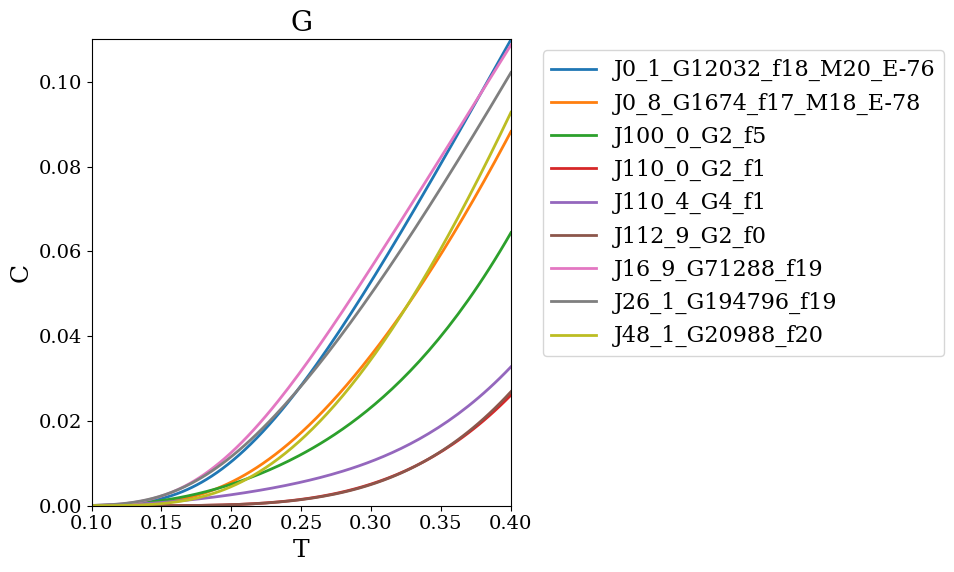
\includegraphics[width=\linewidth]{figs/G}
	\caption{Скорость роста теплоемкости для разных $G$}
	\label{fig:G}
\end{figure}

\begin{figure}[H]
		\centering
		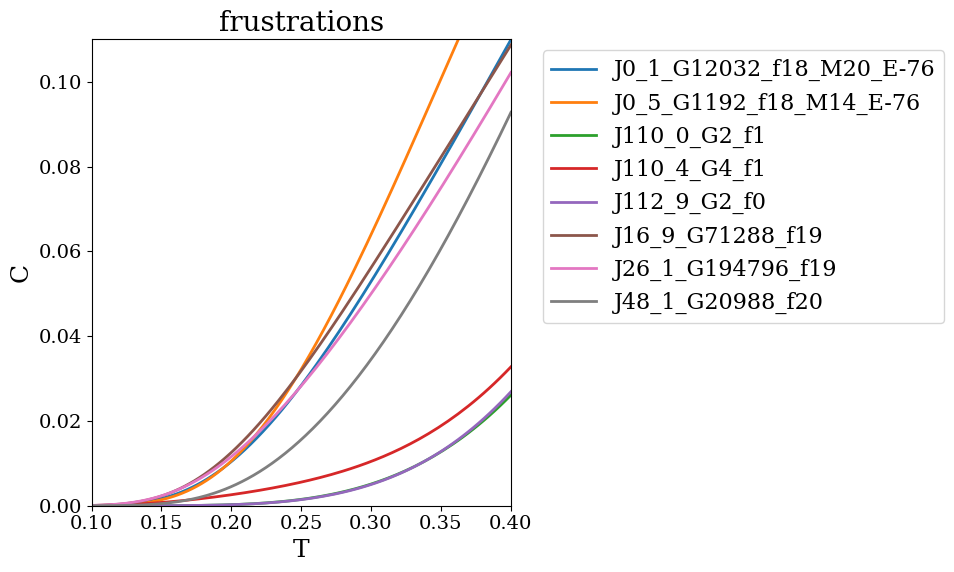
\includegraphics[width=\linewidth]{figs/f}
	\caption{Скорость роста теплоемкости для разных $f$}
	\label{fig:f}
\end{figure}


\begin{figure}[H]
	\centering
	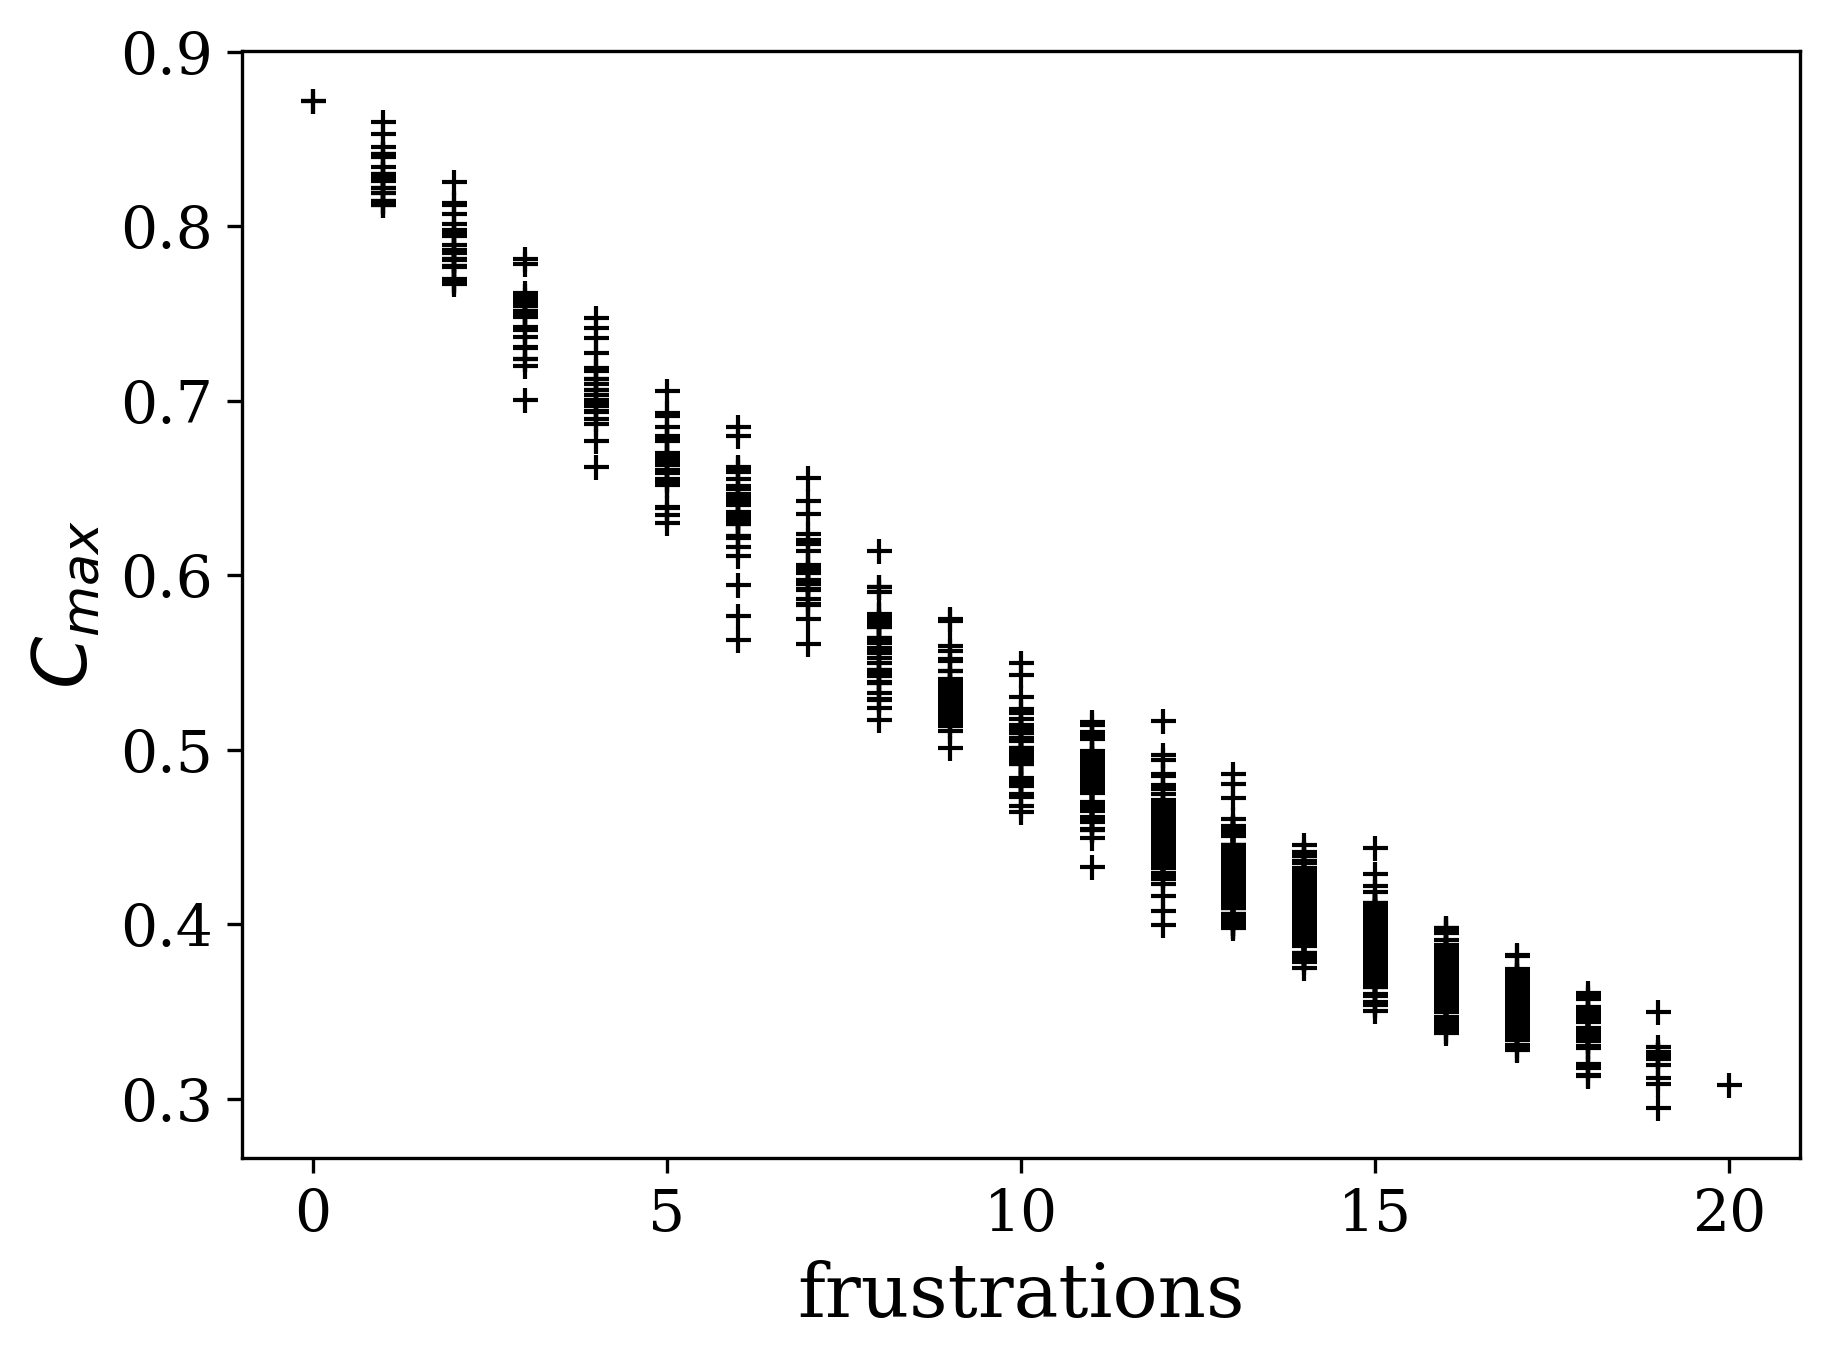
\includegraphics[width=1\textwidth]{figs/C_max(f)}
	\caption{$C_{max(f)}$}
	\label{fig:C_max_f}
\end{figure}


\begin{figure}[H]
	\centering
	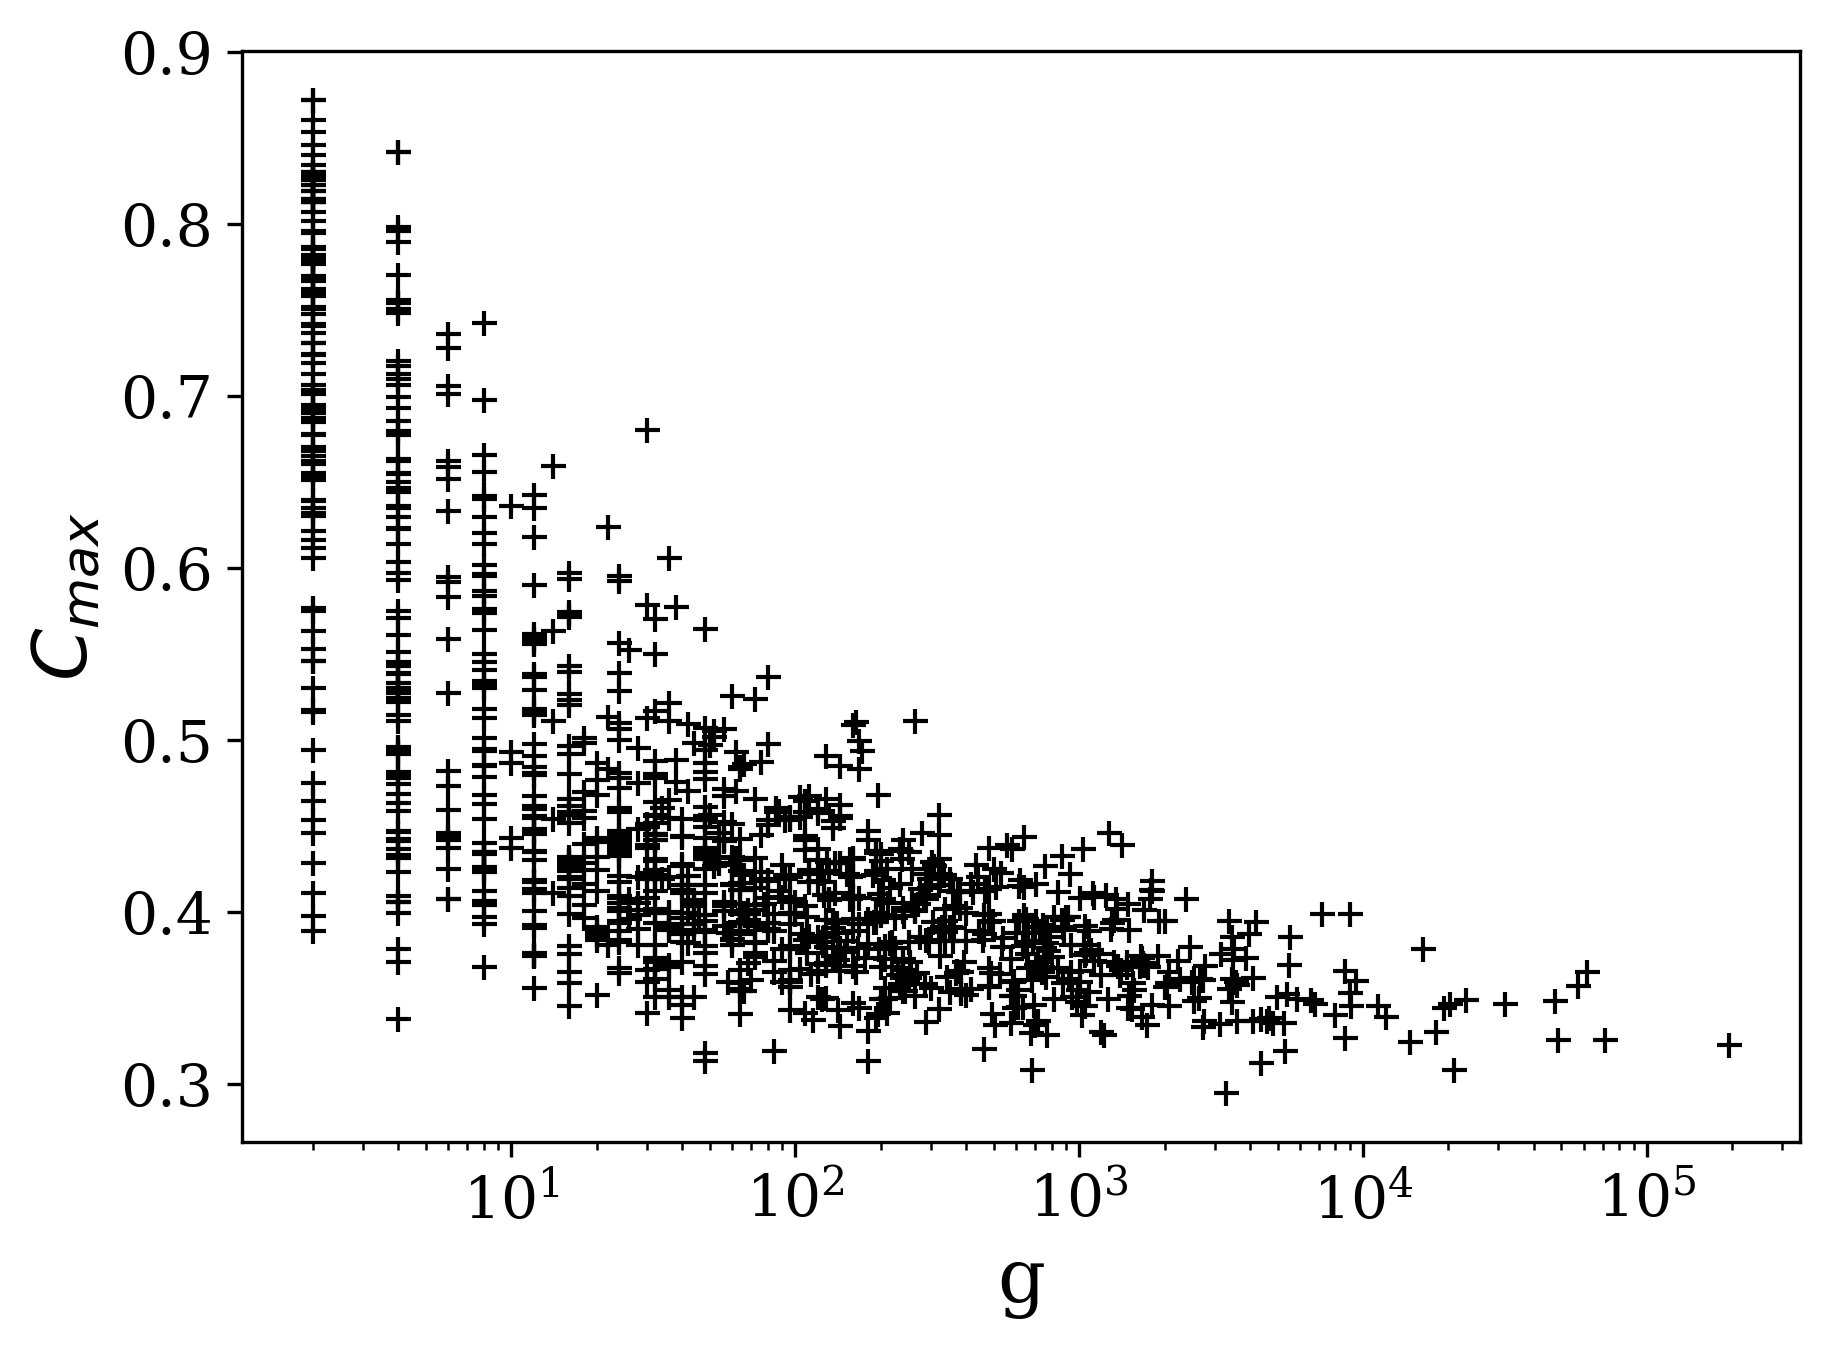
\includegraphics[width=1\textwidth]{figs/C_max(g)}
	\caption{$C_{max(g)}$}
	\label{fig:C_max_g}
\end{figure}

\begin{figure}[H]
	\begin{minipage}{0.5\linewidth}
		\centering
		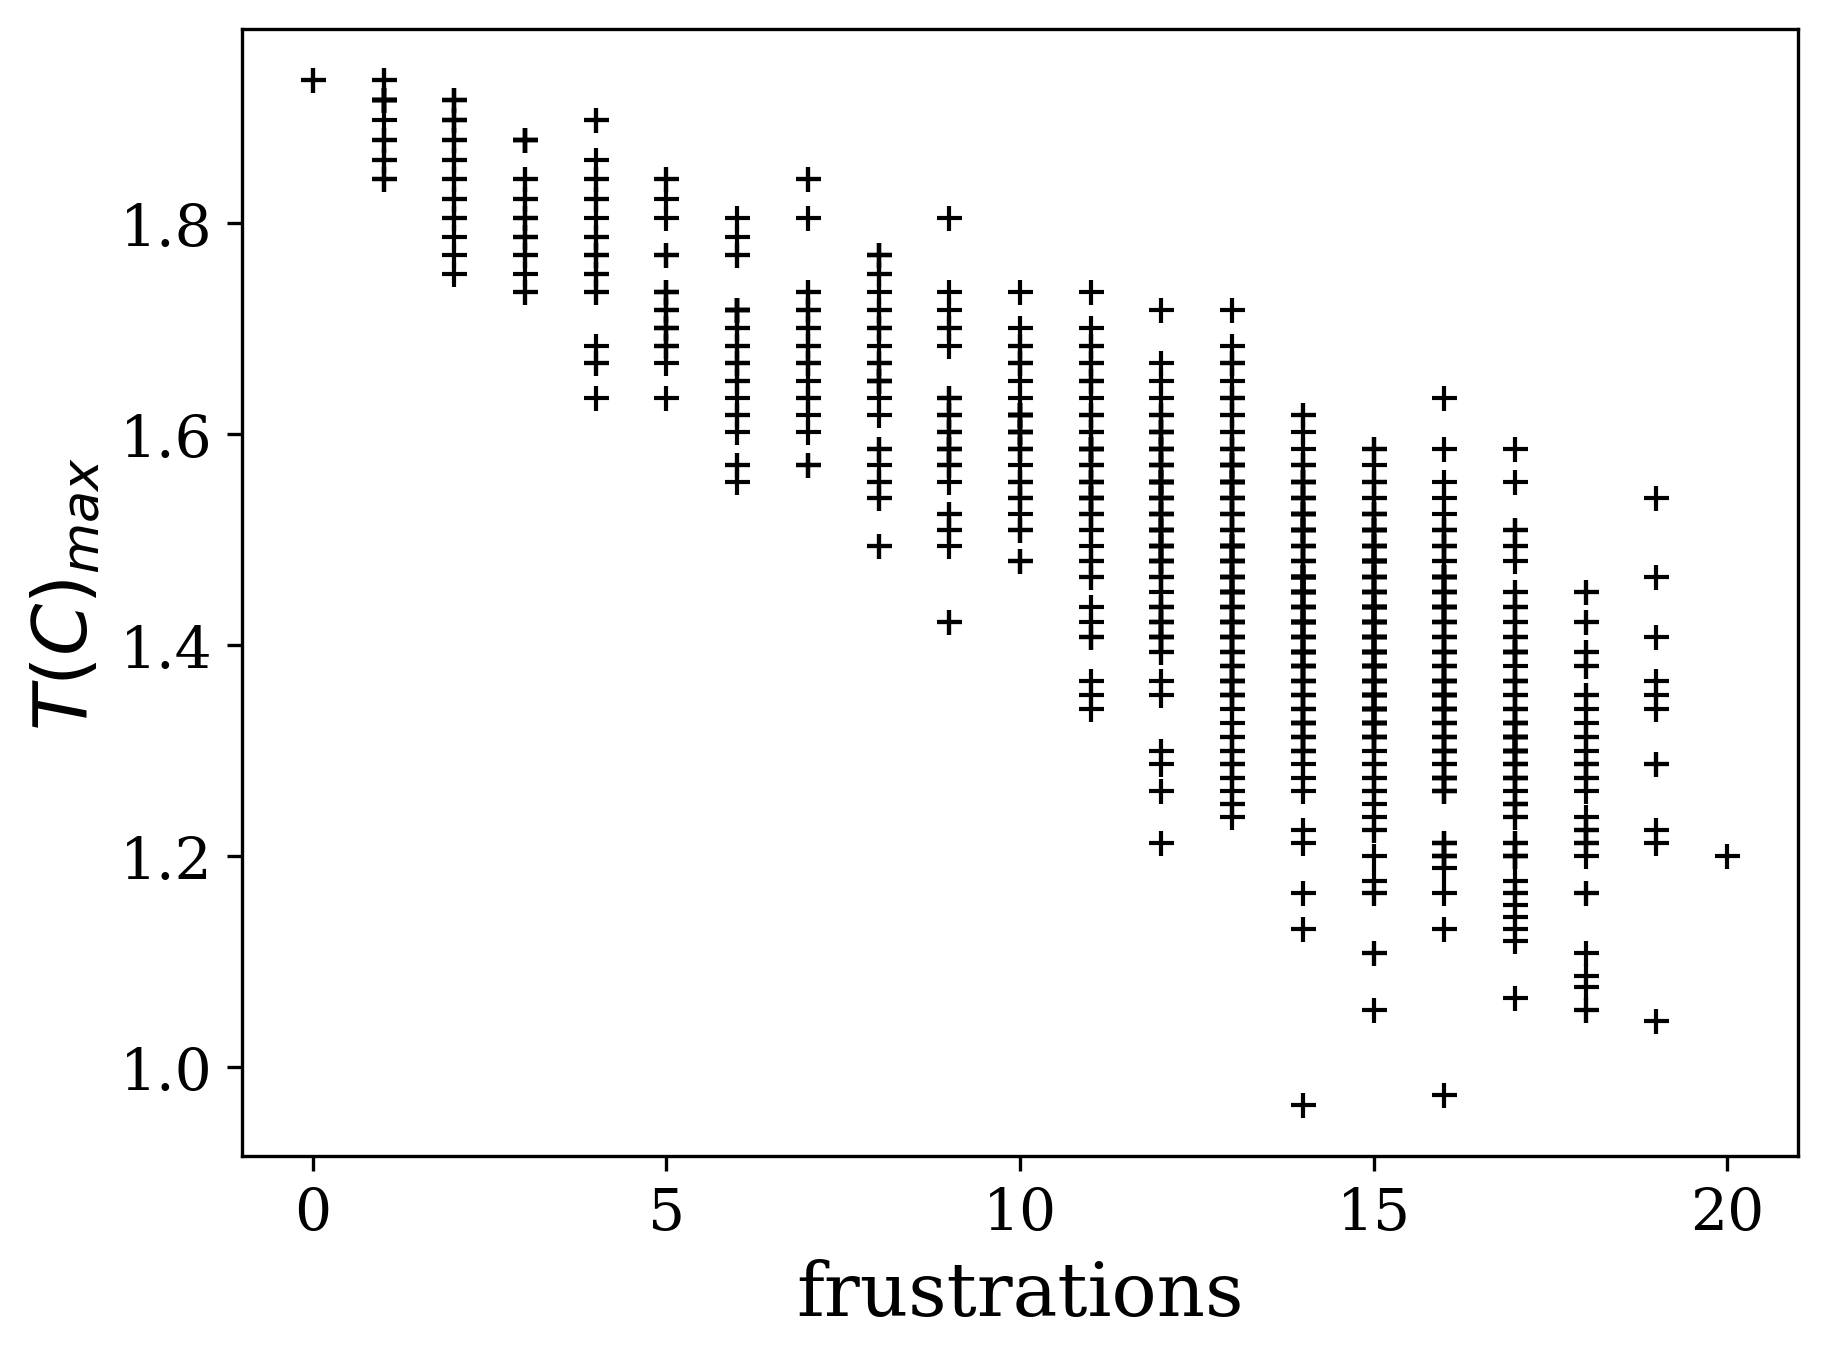
\includegraphics[width=\linewidth]{figs/T_C_max(f)}
	\end{minipage}
	\hfill
	\begin{minipage}{0.5\linewidth}
		\centering
		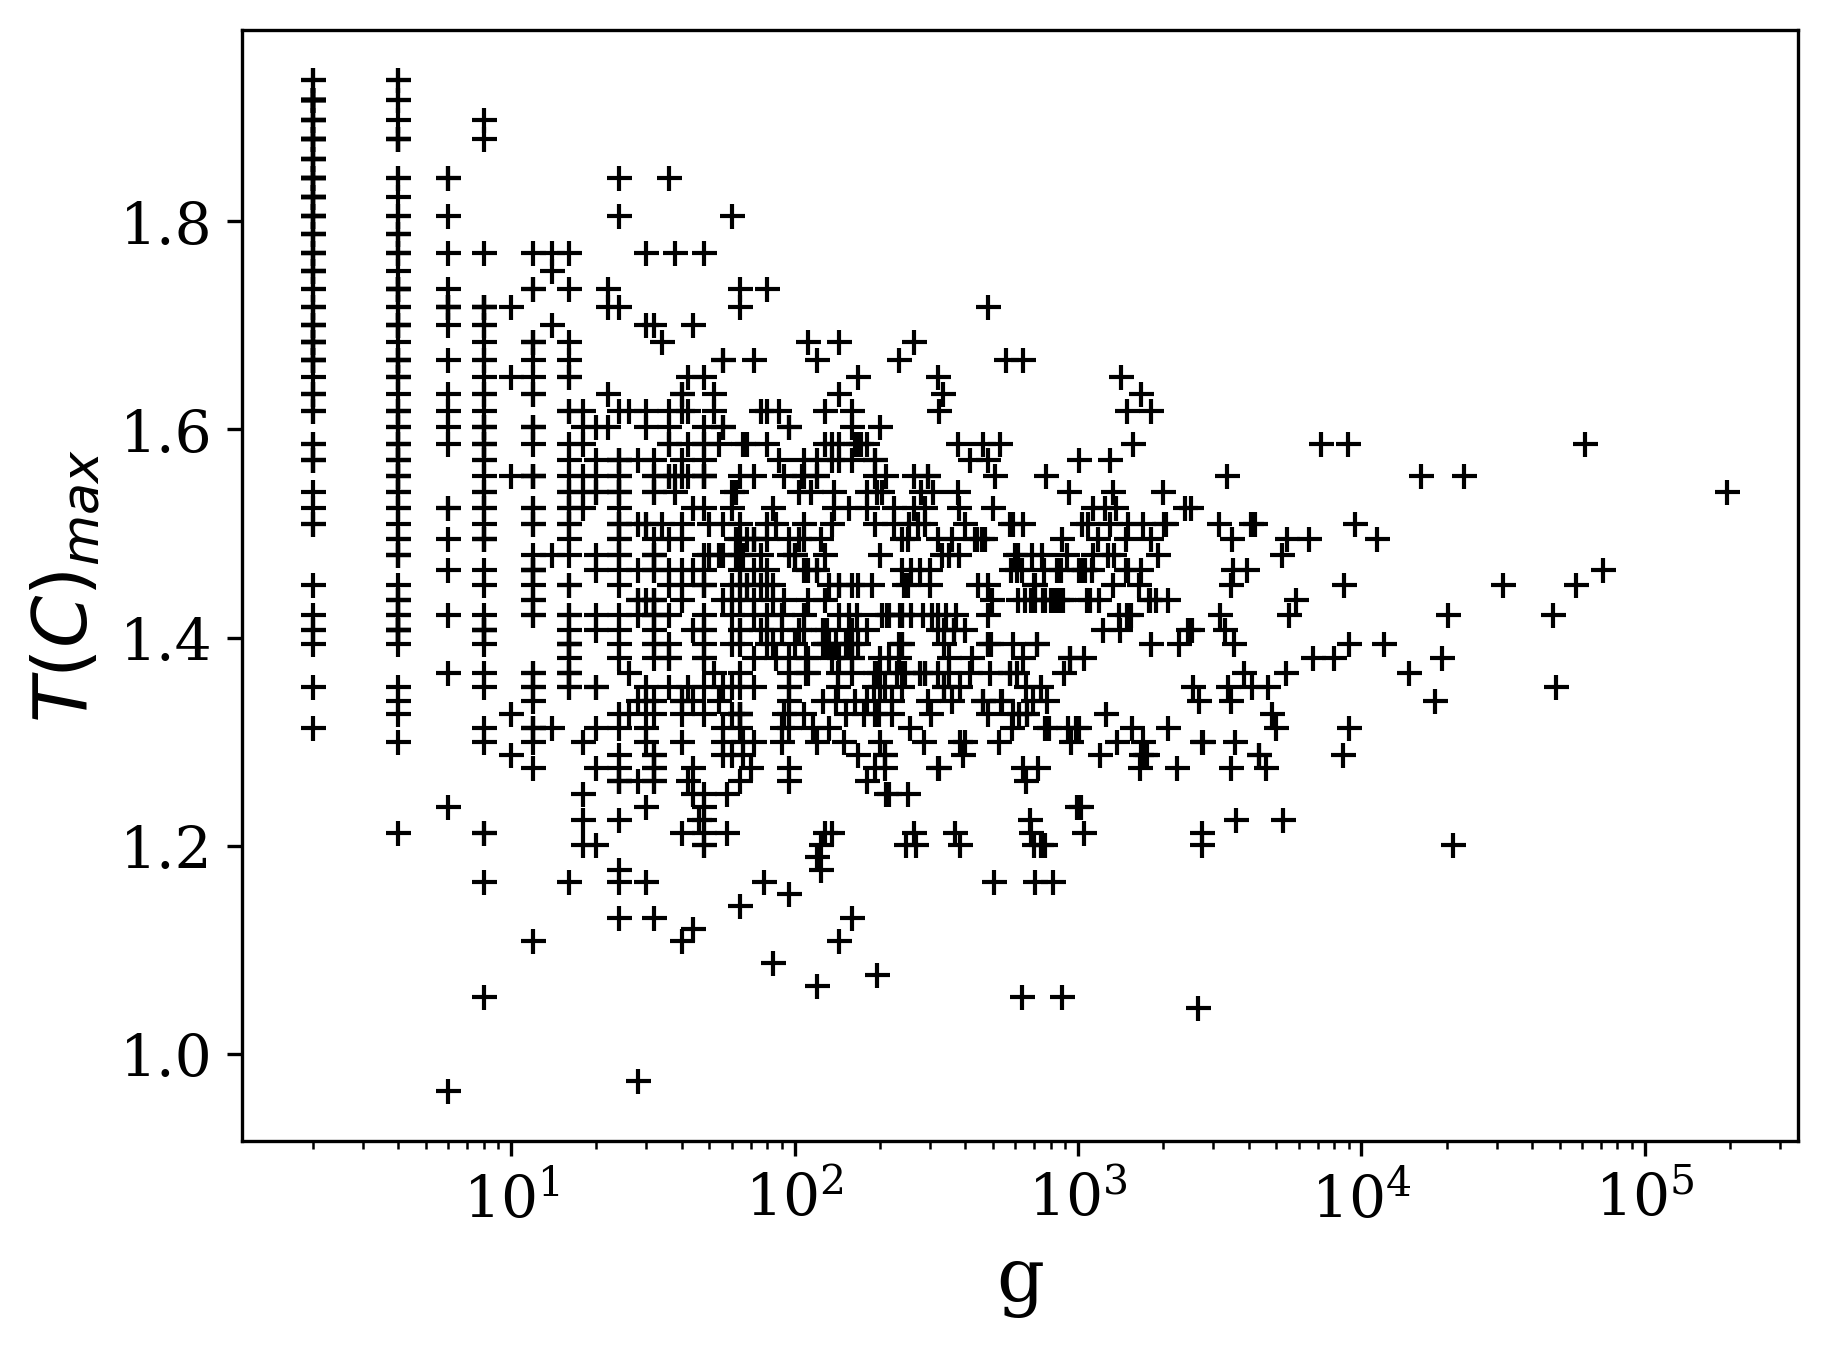
\includegraphics[width=\linewidth]{figs/T_C_max(g)}
	\end{minipage}
	\caption{$T_{C_{max}}$}
	\label{fig:T_C_max}
\end{figure}

\begin{figure}[H]
	\begin{minipage}{0.5\linewidth}
		\centering
		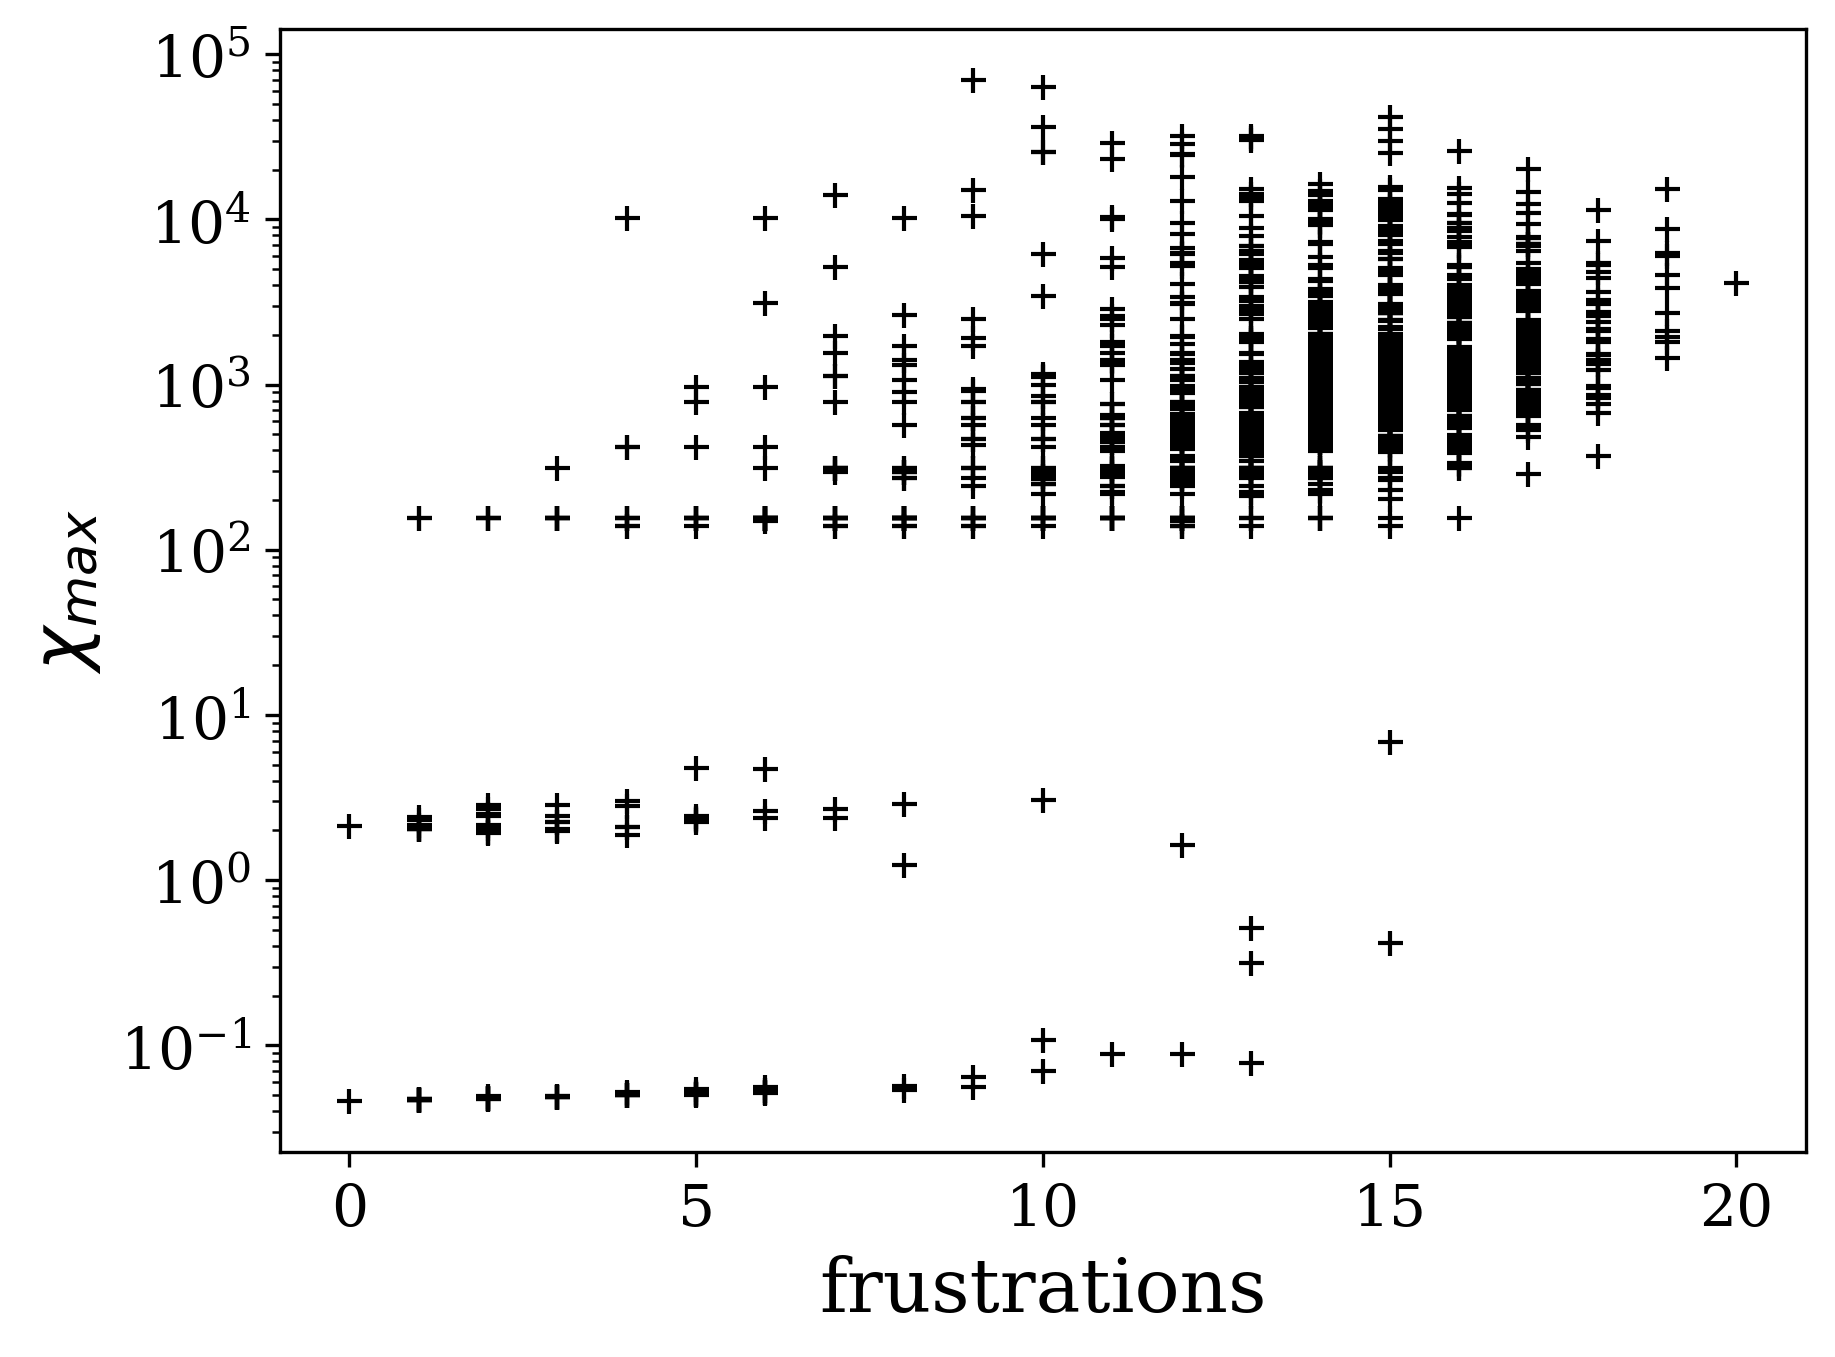
\includegraphics[width=\linewidth]{figs/chi_max(f)}
	\end{minipage}
	\hfill
	\begin{minipage}{0.5\linewidth}
		\centering
		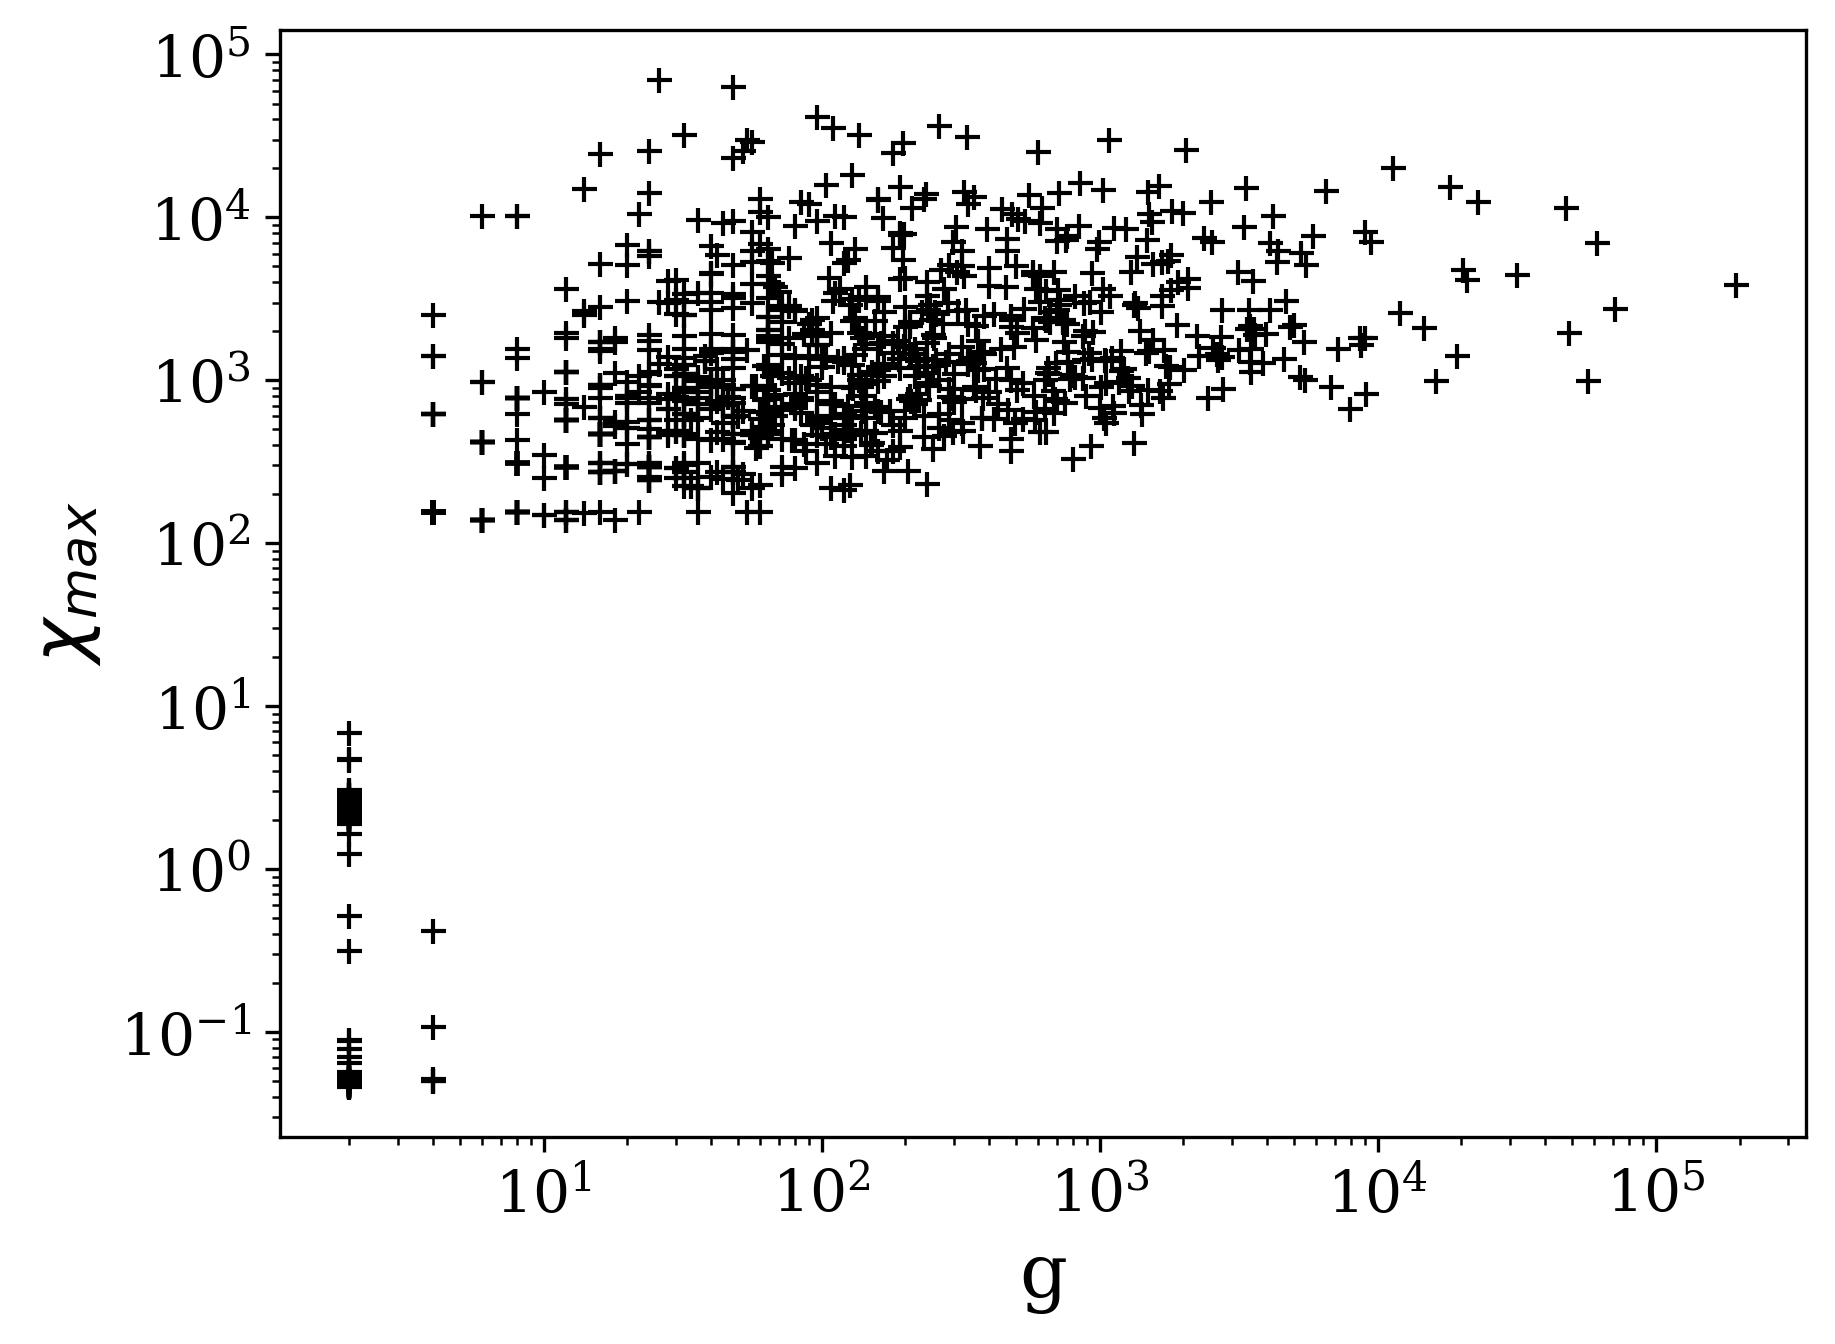
\includegraphics[width=\linewidth]{figs/chi_max(g)}
	\end{minipage}
	\caption{$\chi_{max}$}
	\label{fig:chi_max}
\end{figure}

\begin{figure}[H]
	\begin{minipage}{0.5\linewidth}
		\centering
		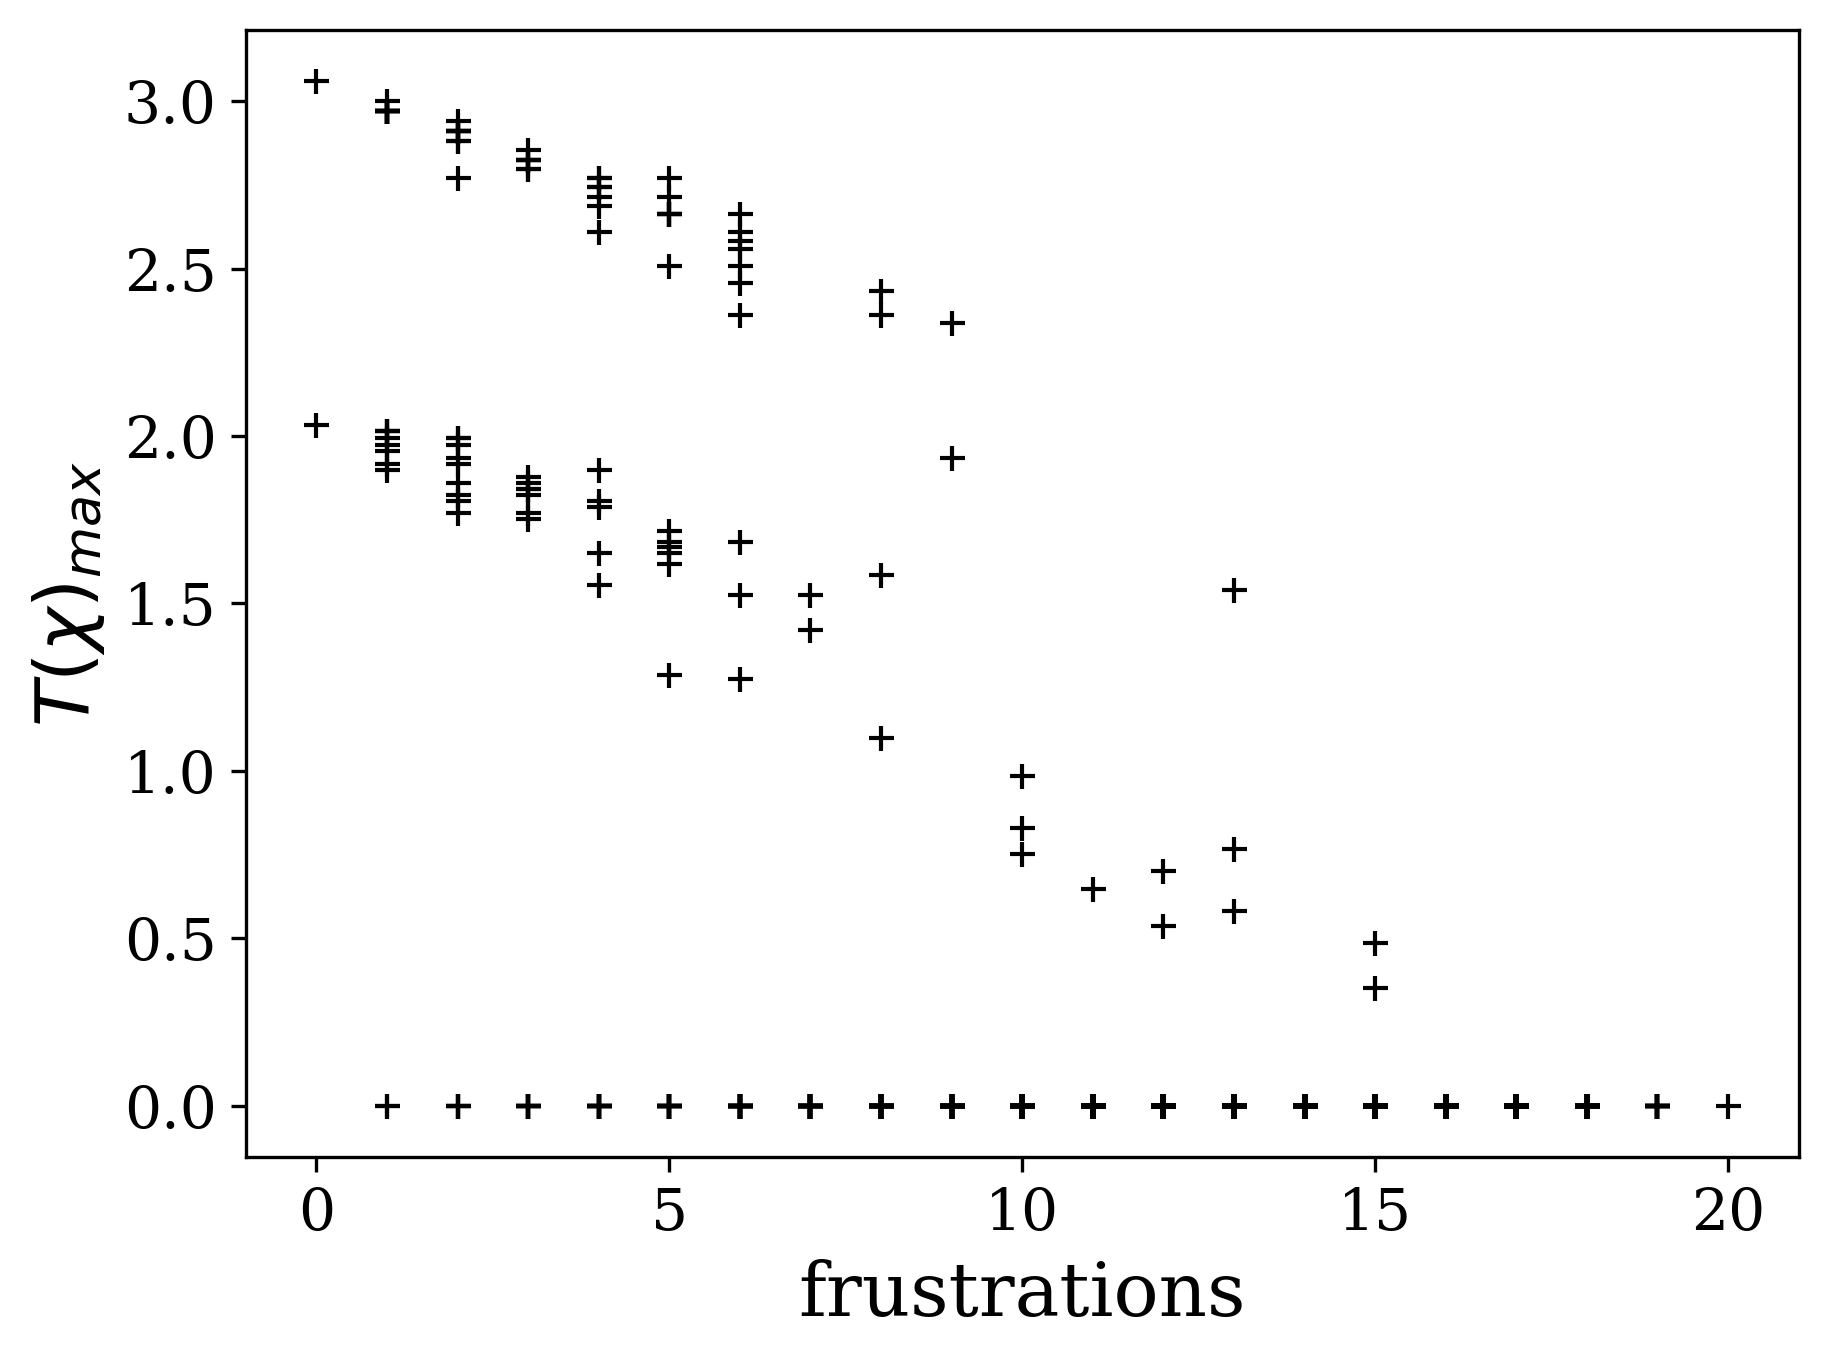
\includegraphics[width=\linewidth]{figs/T_chi_max(f)}
	\end{minipage}
	\hfill
	\begin{minipage}{0.5\linewidth}
		\centering
		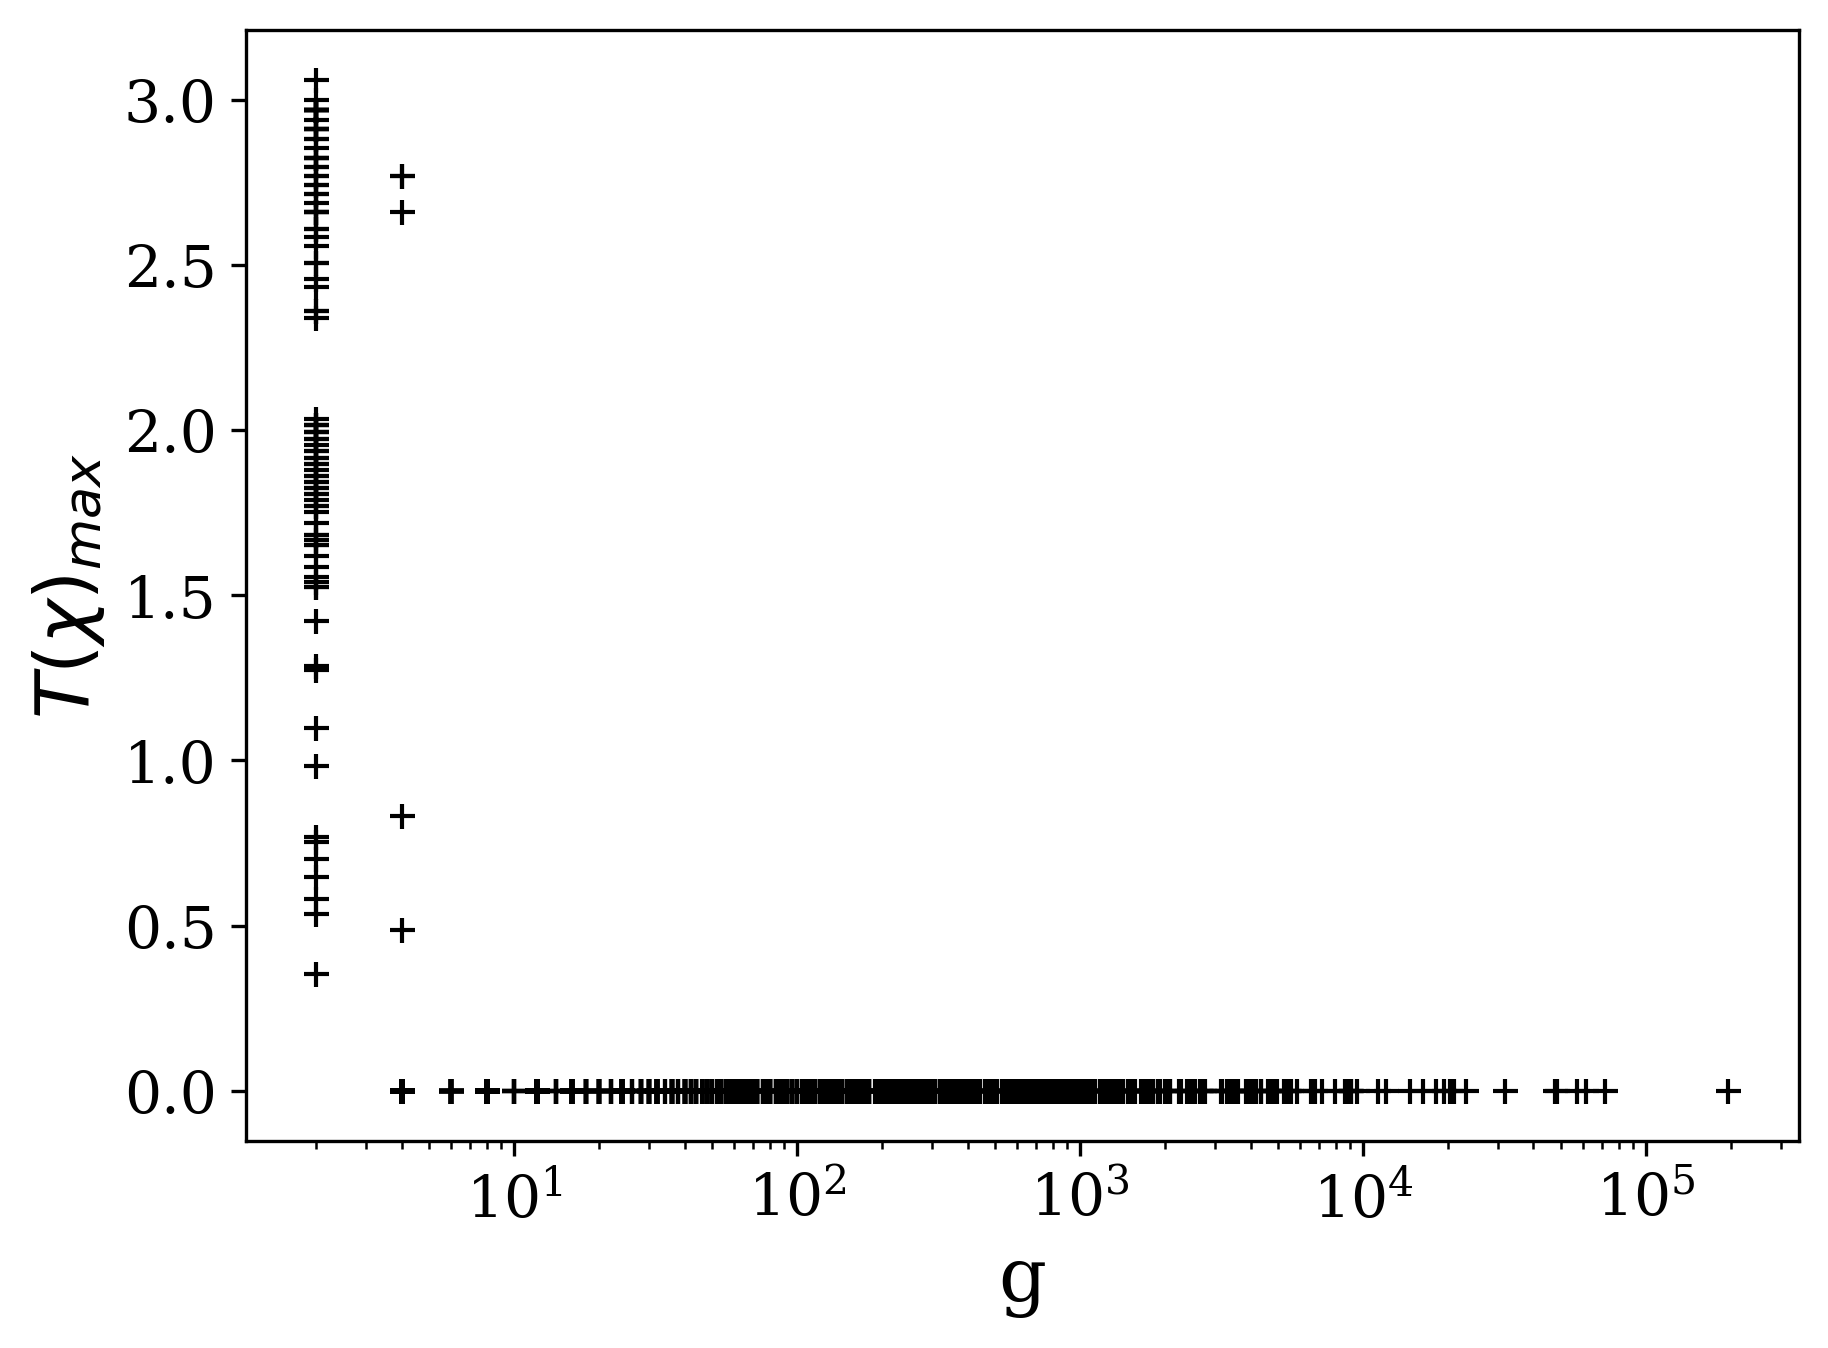
\includegraphics[width=\linewidth]{figs/T_chi_max(g)}
	\end{minipage}
	\caption{$T_{\chi_{max}}$}
	\label{fig:T_chi_max}
\end{figure}

\begin{figure}[H]
	\begin{minipage}{0.5\linewidth}
		\centering
		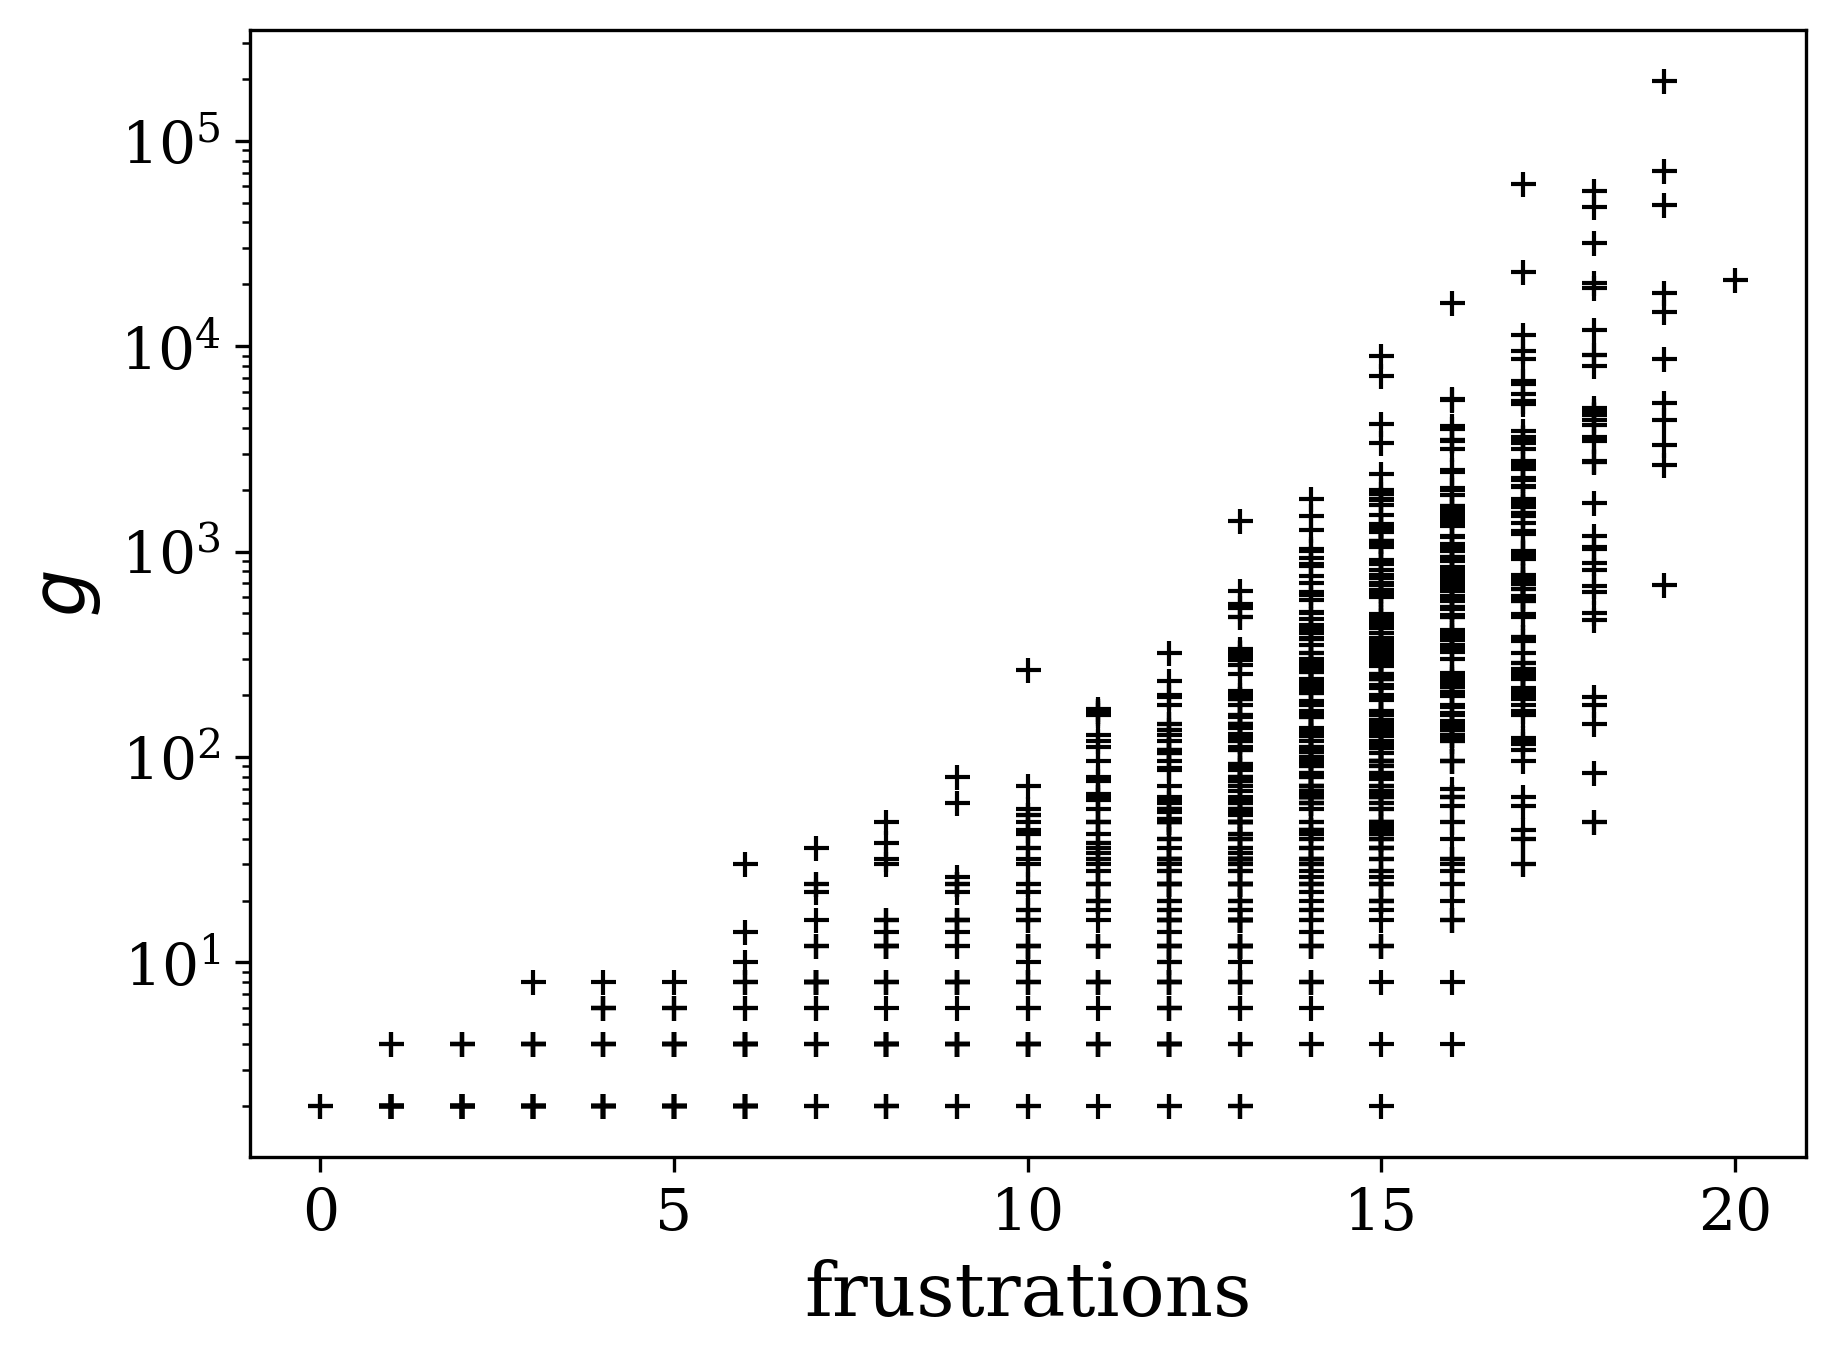
\includegraphics[width=\linewidth]{figs/g(f)}
	\end{minipage}
	\hfill
	\begin{minipage}{0.5\linewidth}
		\centering
		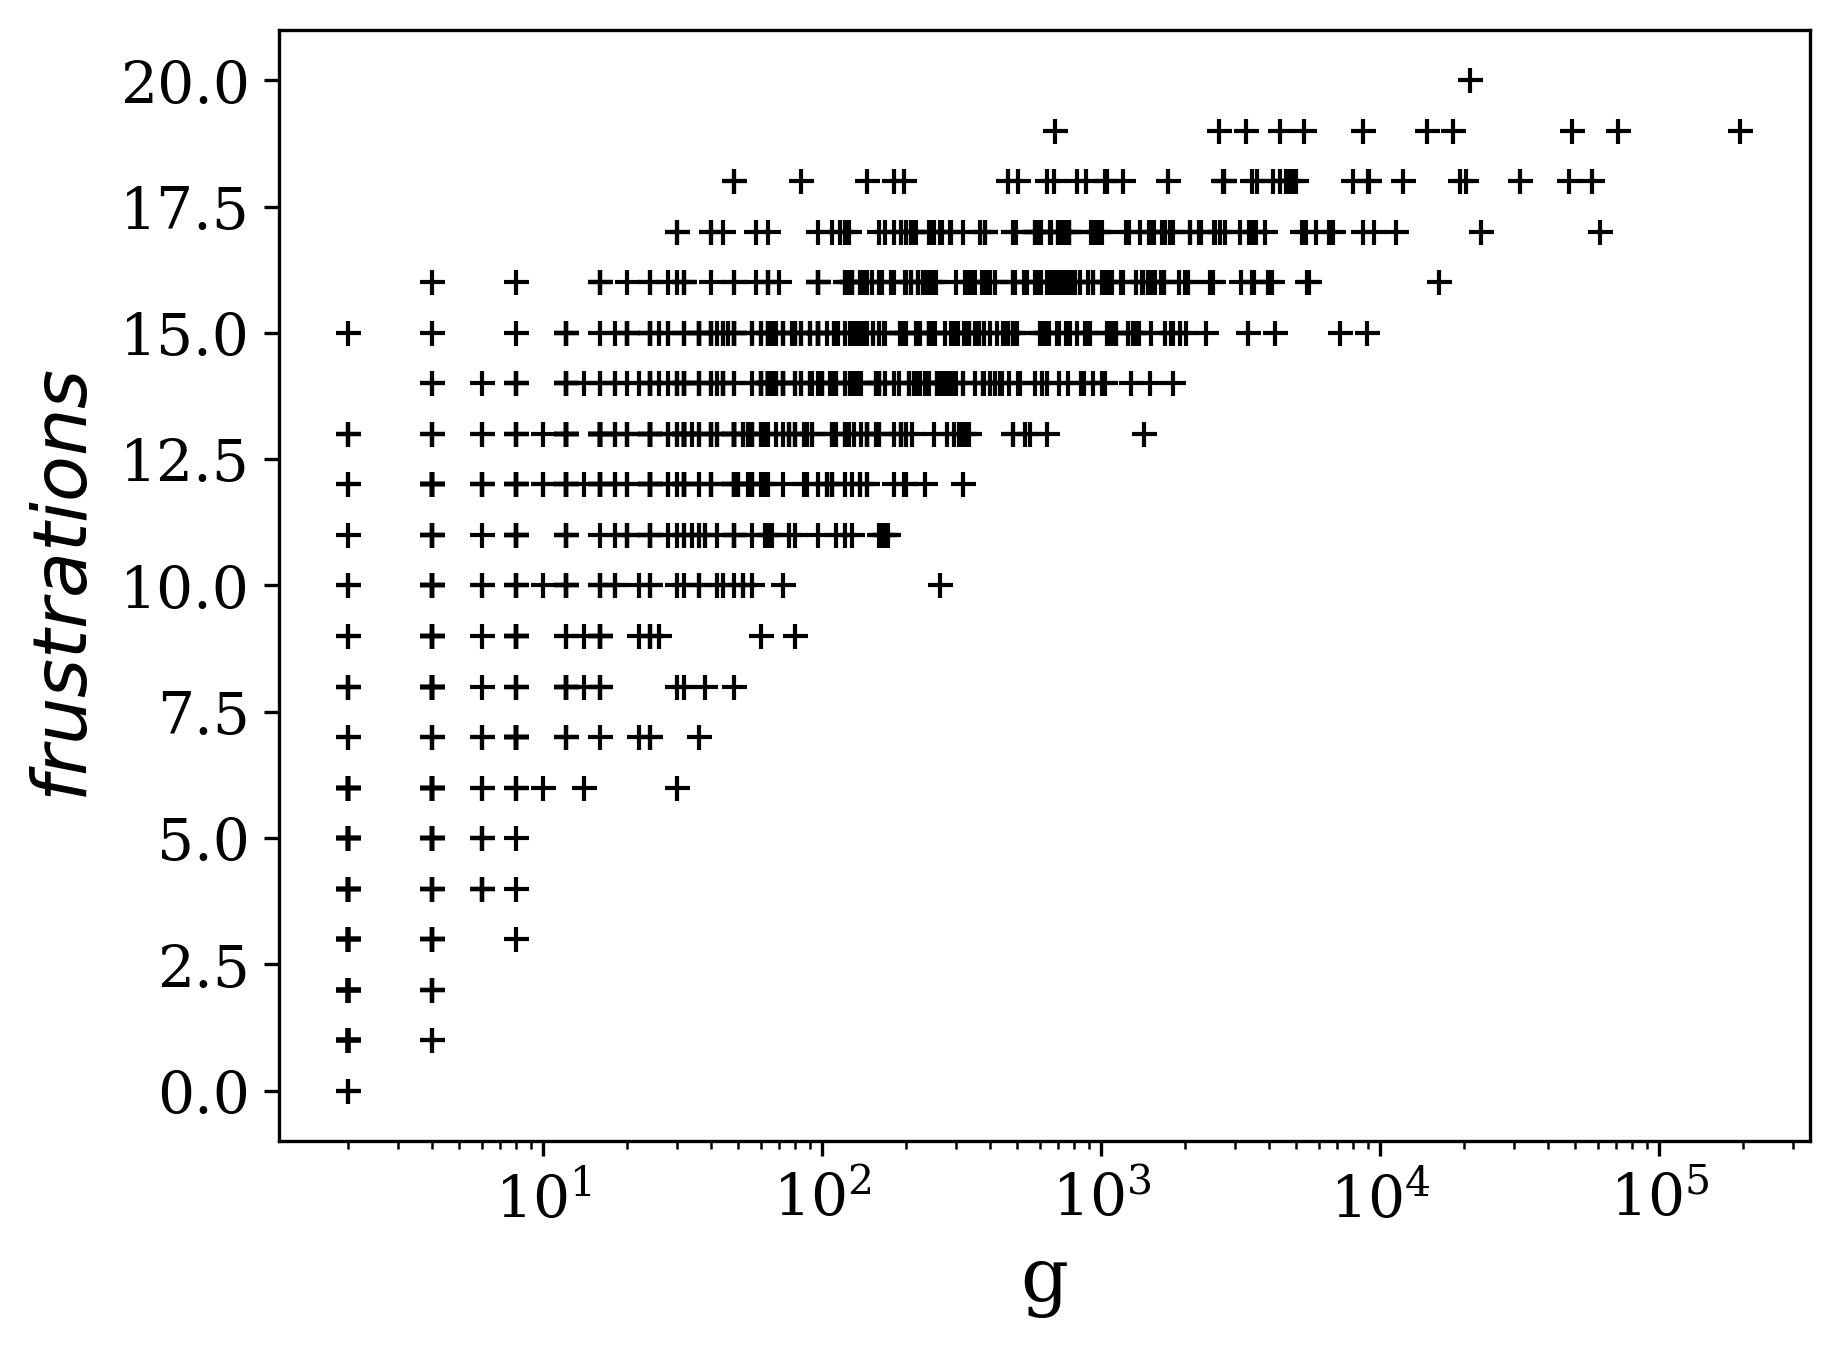
\includegraphics[width=\linewidth]{figs/f(g)}
	\end{minipage}
	\caption{$g$ and $f$}
	\label{fig:g_f}
\end{figure}


\begin{figure}[H]
	\centering
	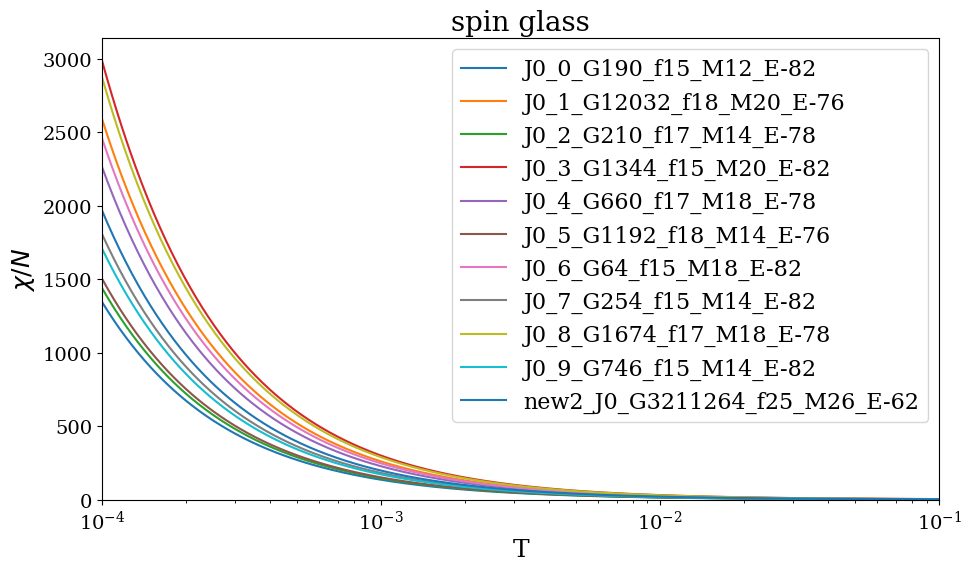
\includegraphics[width=1\textwidth]{figs/spin_glass}
	\caption{spin glass}
	\label{fig:spin_glass}
\end{figure}

\begin{figure}[H]
	\centering
	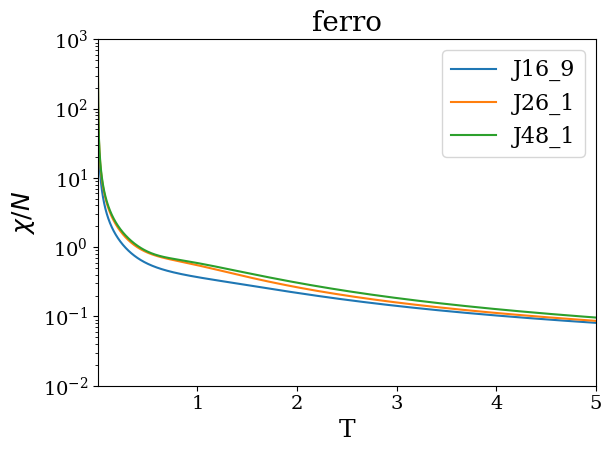
\includegraphics[width=1\textwidth]{figs/ferro1}
	\caption{ferro1}
	\label{fig:ferro1}
\end{figure}

\begin{figure}[H]
	\centering
	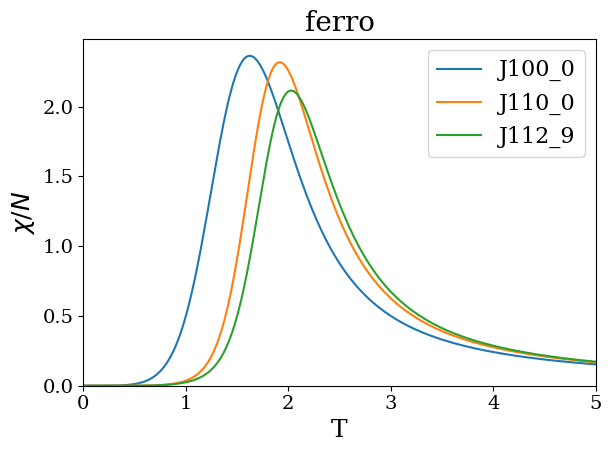
\includegraphics[width=1\textwidth]{figs/ferro2}
	\caption{ferro2}
	\label{fig:ferro2}
\end{figure}

\begin{figure}[H]
	\centering
	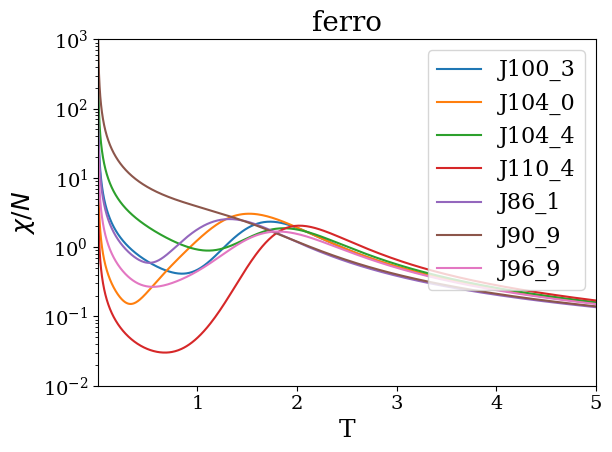
\includegraphics[width=1\textwidth]{figs/ferro3}
	\caption{ferro3}
	\label{fig:ferro3}
\end{figure}

\begin{figure}[H]
	\centering
	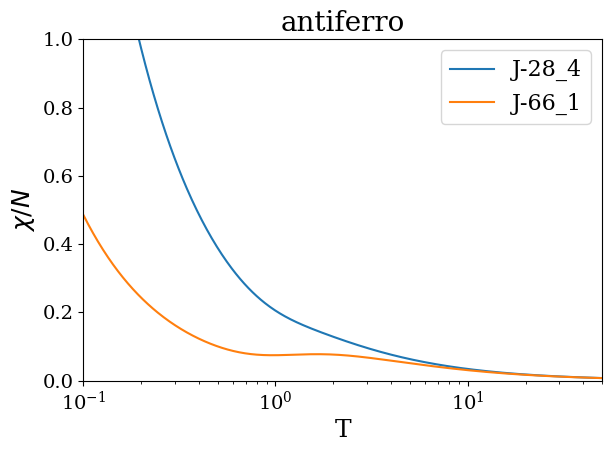
\includegraphics[width=1\textwidth]{figs/antiferro1}
	\caption{antiferro1}
	\label{fig:antiferro1}
\end{figure}

\begin{figure}[H]
	\centering
	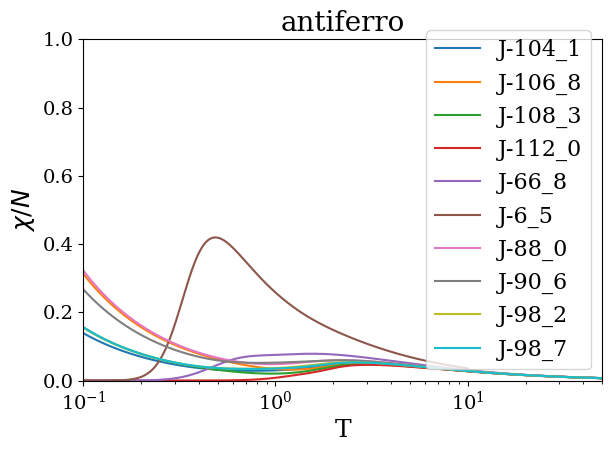
\includegraphics[width=1\textwidth]{figs/antiferro2}
	\caption{antiferro2}
	\label{fig:antiferro2}
\end{figure}

\section{Магнитный структурный фактор конфигураций основного состояния}
Для различных конфигураций основного состояния спинового стекла Эдвардса-Андерсон, полученных алгоритмом Метрополиса-Гастингса \cite{metropolis1953equation} и подтвержденных точным расчетом плотности состояний \cite{trukhin2025low}, был рассчитан магнитный структурный фактор через Фурье-образ спин-спиновых корреляционных функций скалярных переменных Изинга:
\begin{equation}     
	I(\vec{q}) = \frac{1}{N} \sum_{i=1}^{N} \sum_{j=1}^{N} S_i S_j \exp(i \vec{q} \cdot \vec{r}_{ij})    
	 \label{eq:I_q_double_sum} 
\end{equation}
где $\vec{q}$ -- вектор рассеяния.

\begin{figure}[H]
	\begin{minipage}{0.5\linewidth}
		\centering
		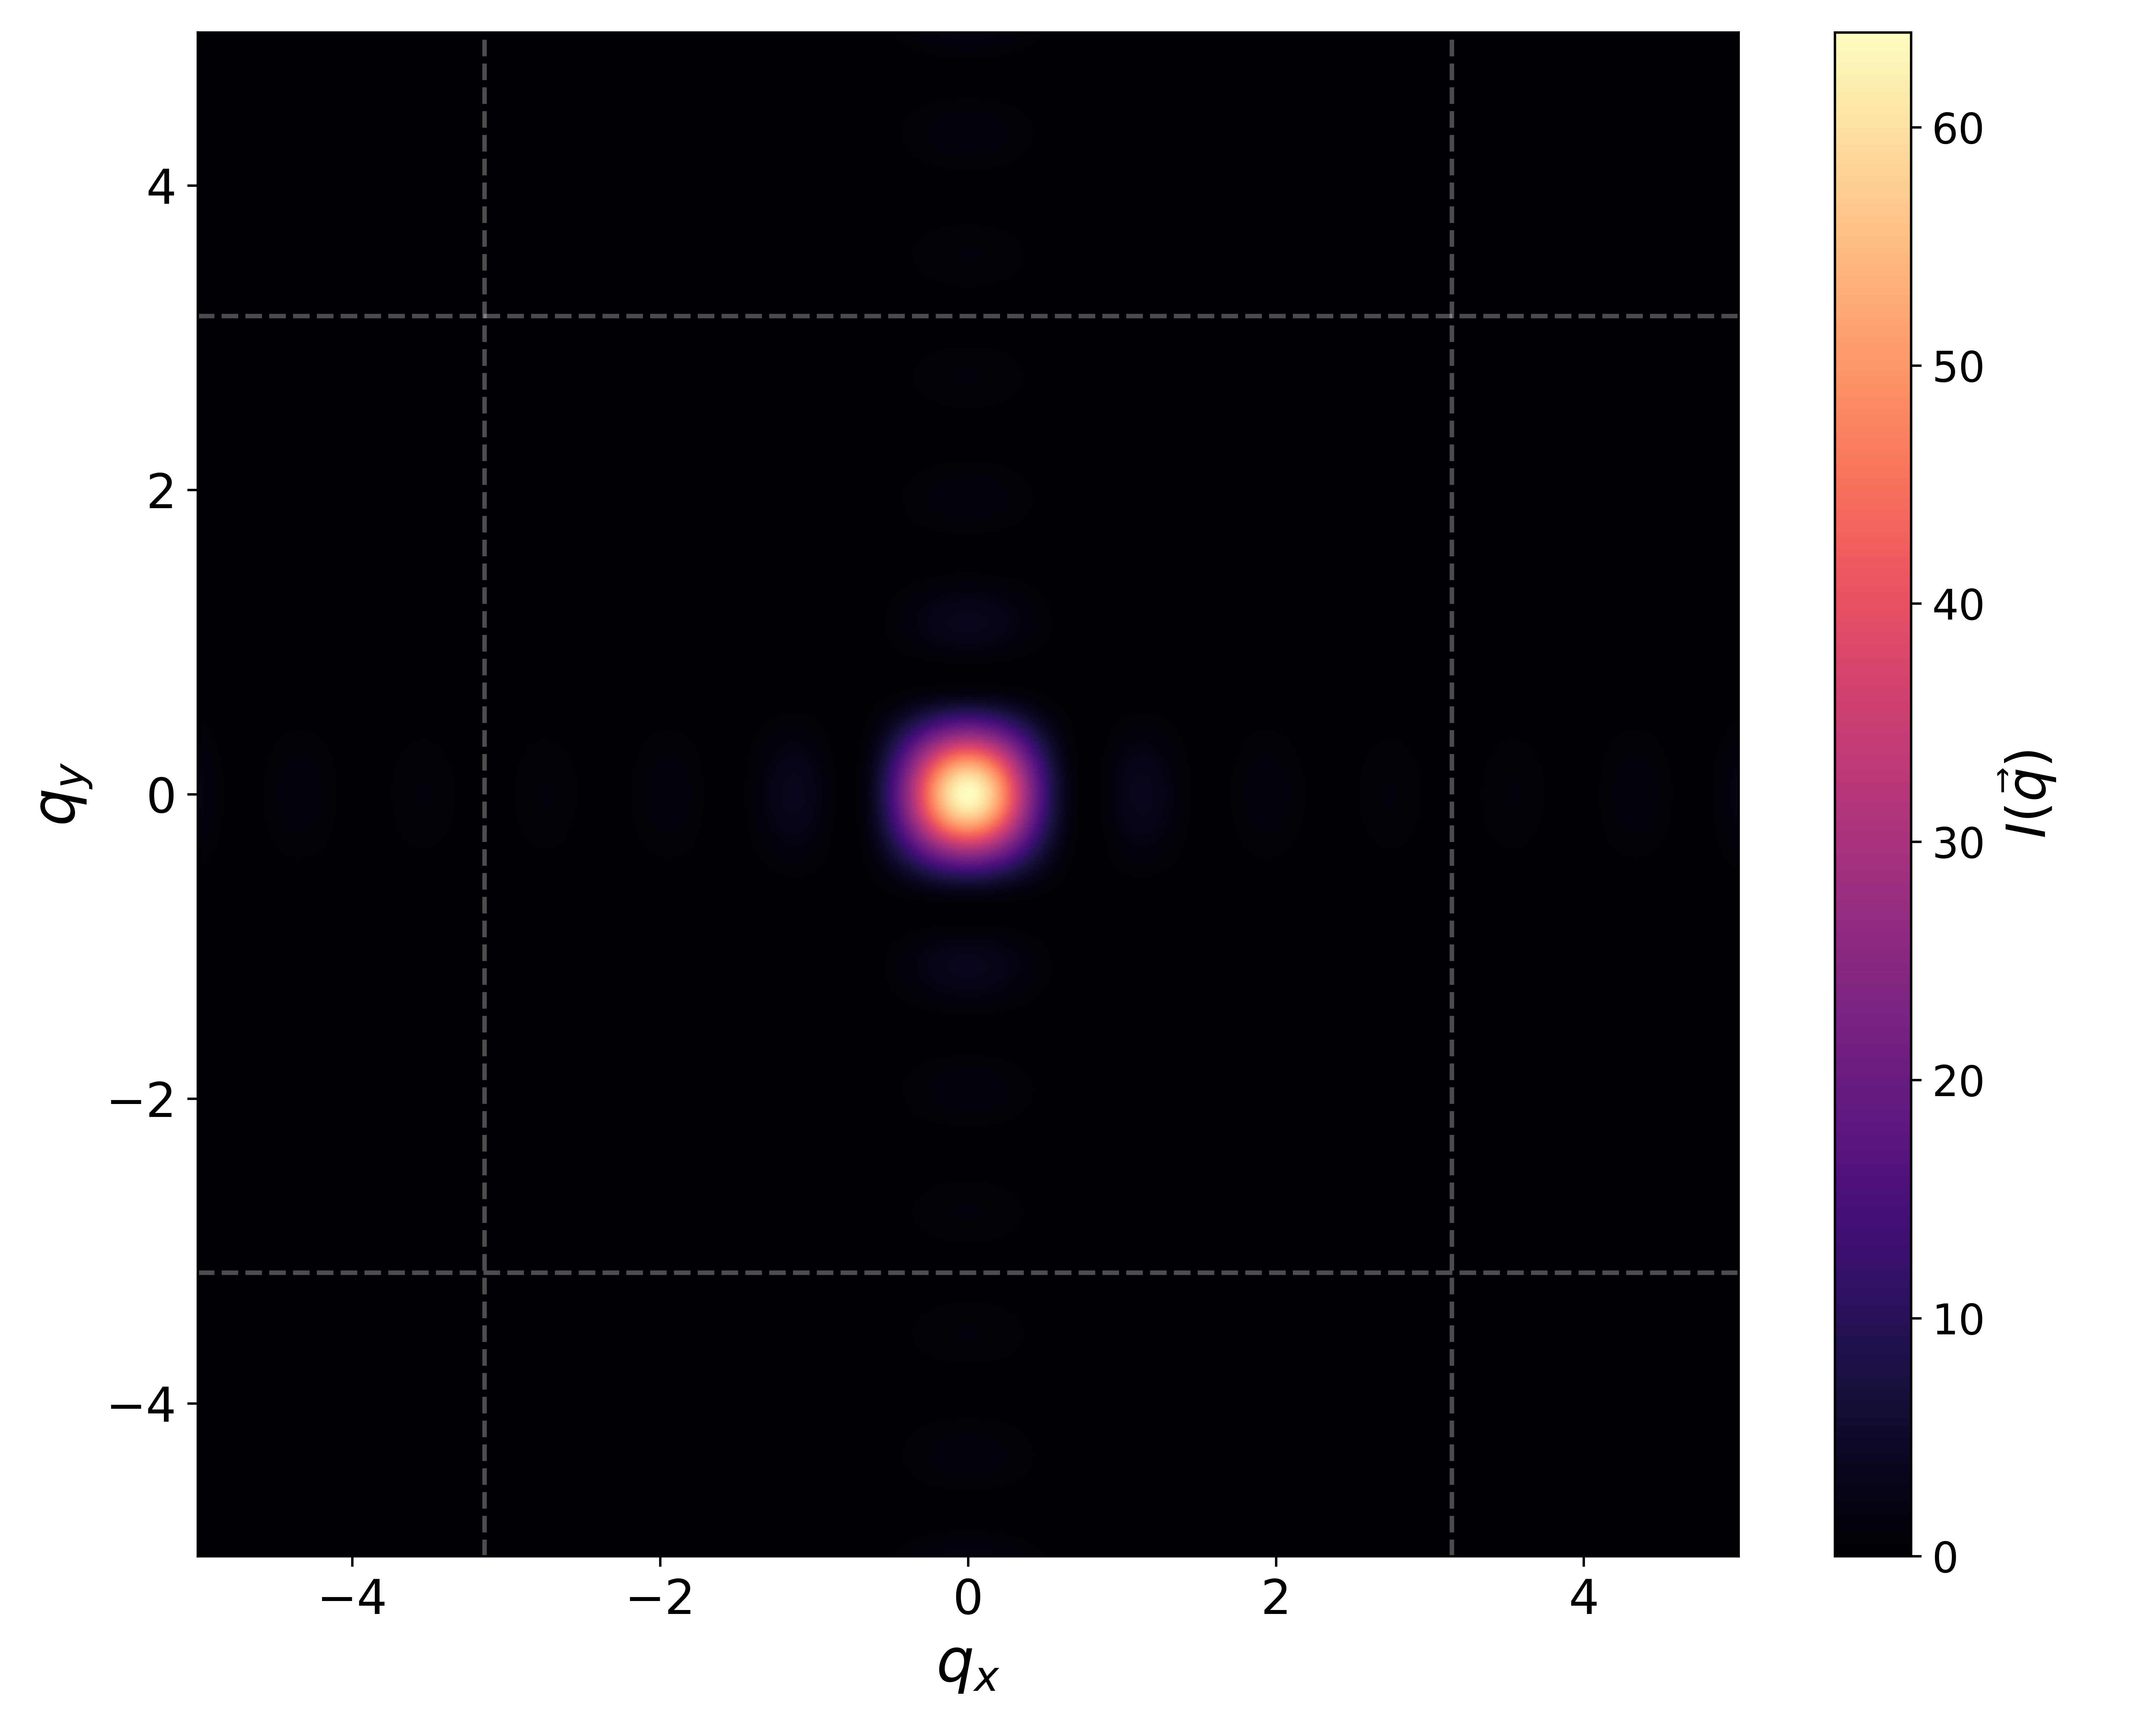
\includegraphics[width=\linewidth]{figs/cell64_J112_9_config_1_msf}
	\end{minipage}
	\hfill
	\begin{minipage}{0.5\linewidth}
		\centering
		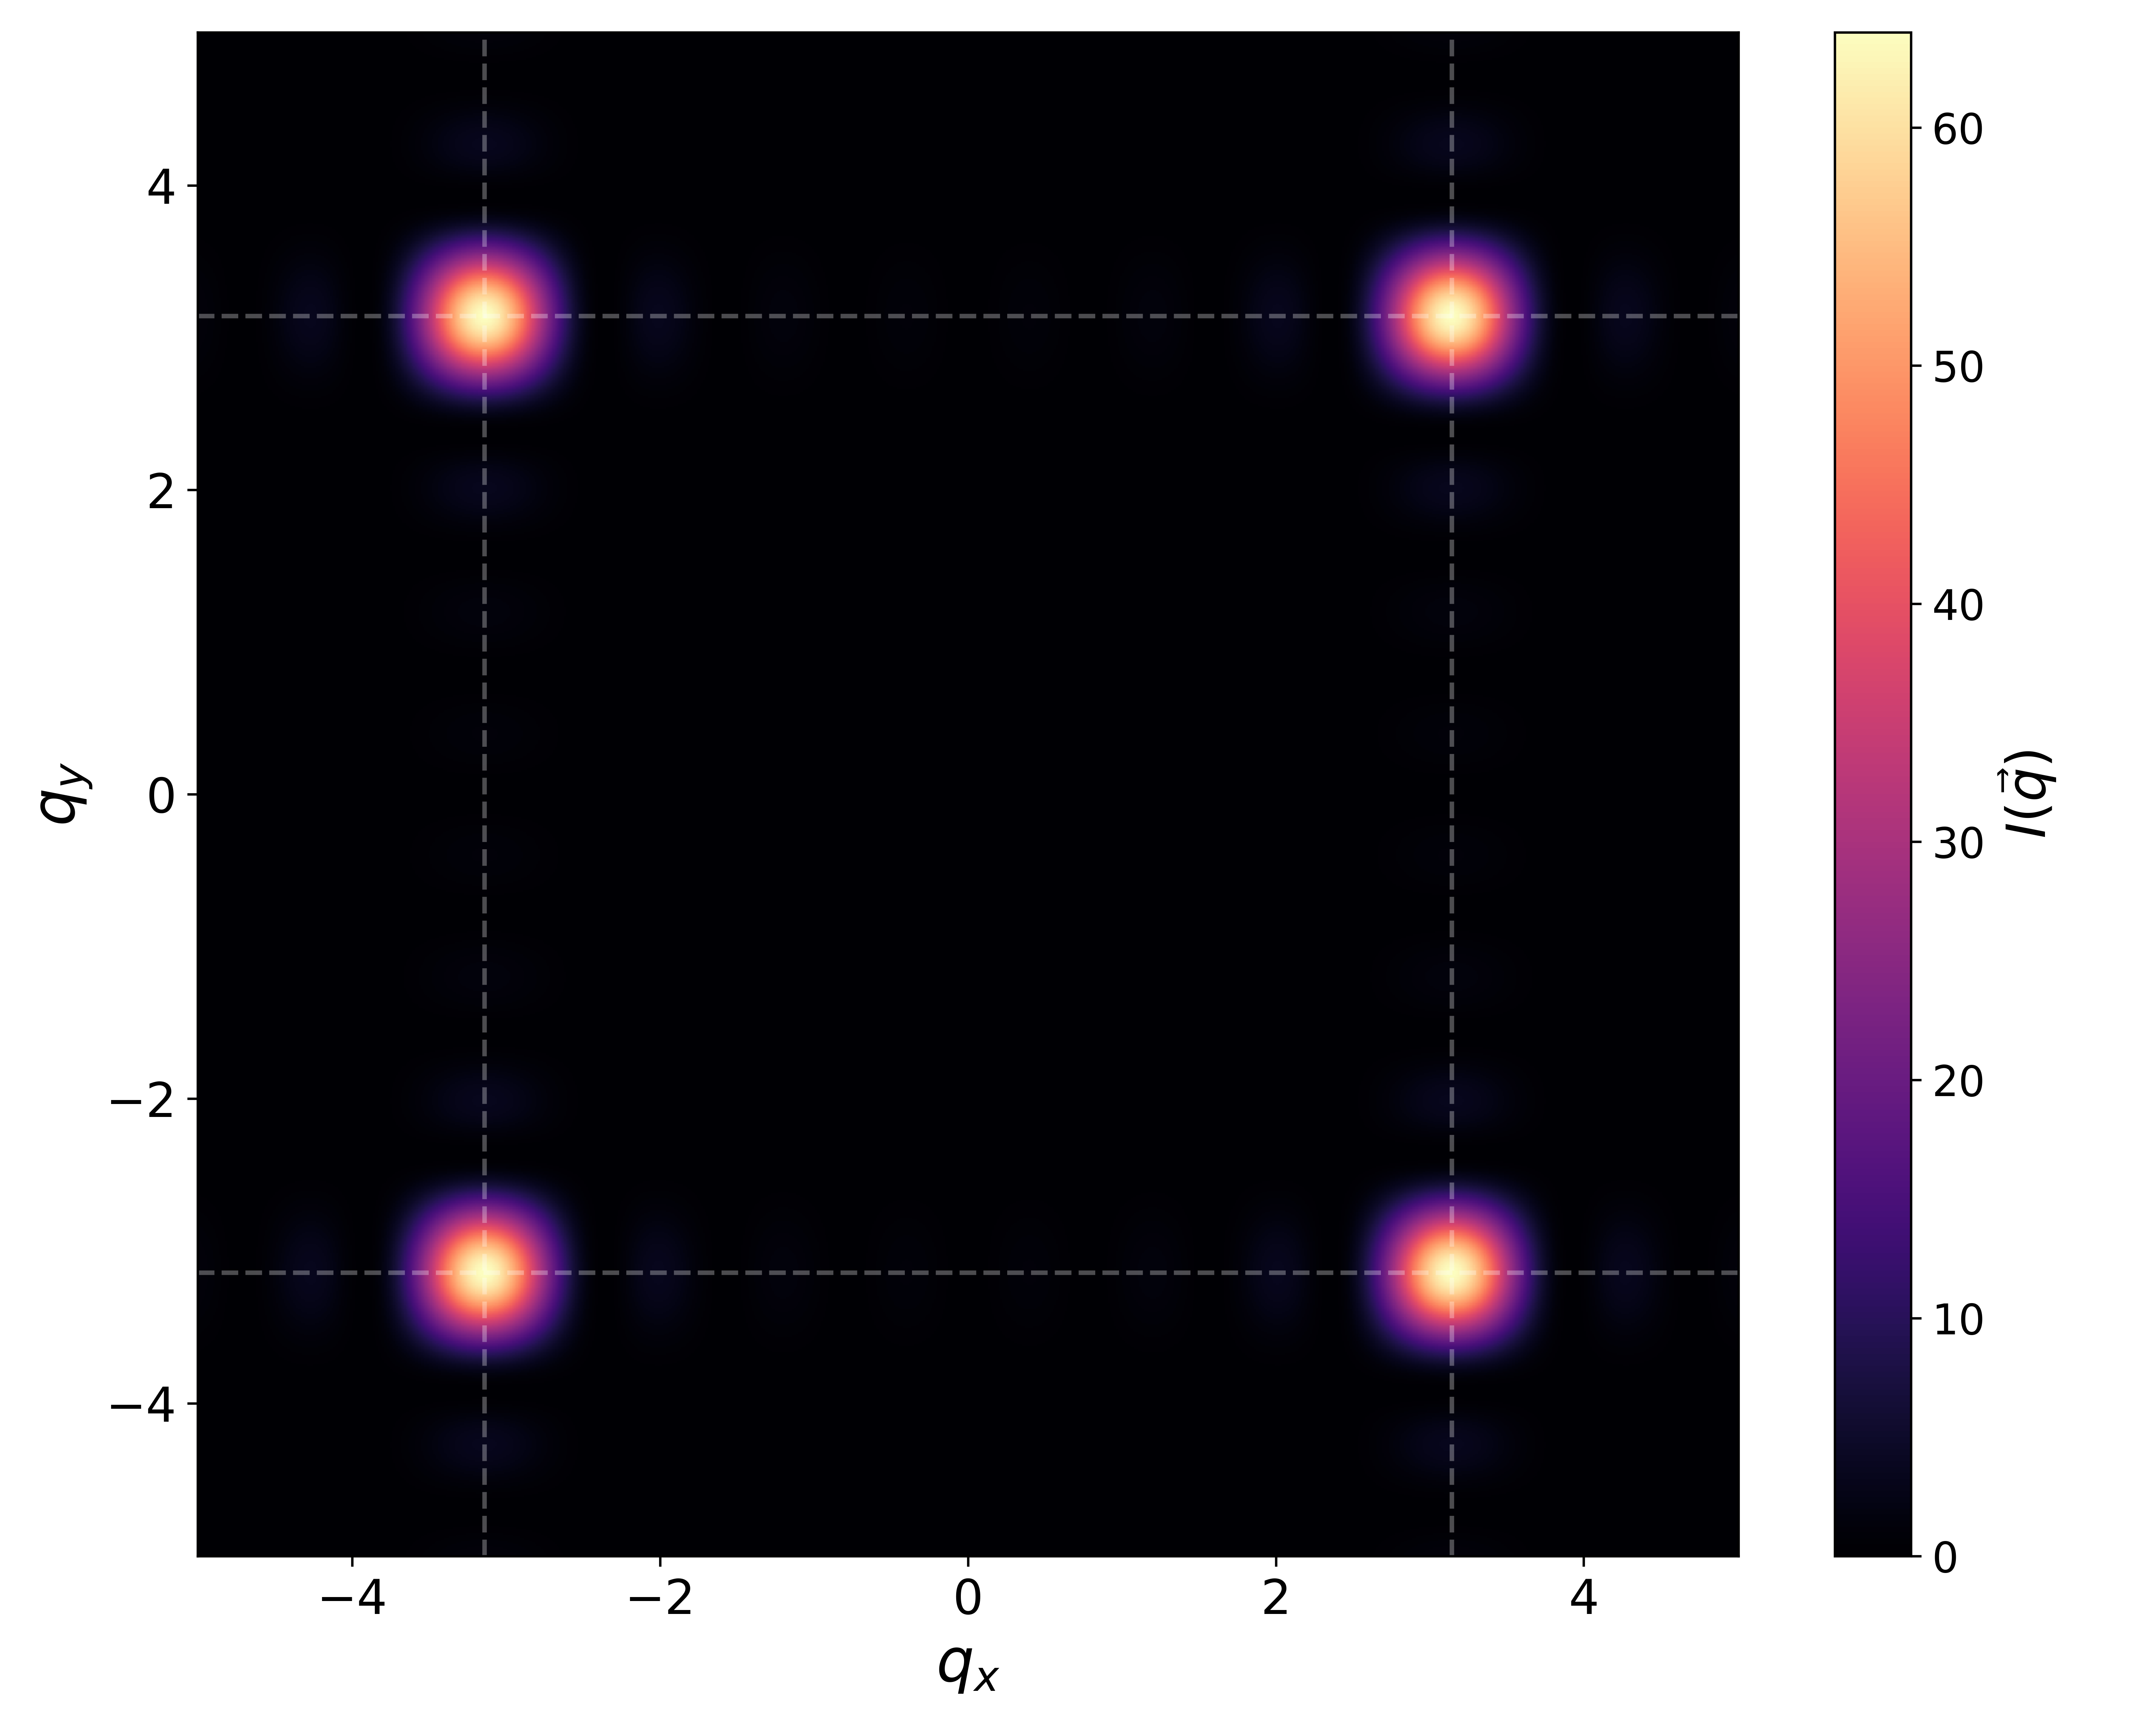
\includegraphics[width=\linewidth]{figs/cell64_J-112_0_config_1_msf}
	\end{minipage}
	\caption{Магнитный структурный фактор $I(\vec{q})$ для ферромагнитного (слева) и антиферромагнитного (справа) упорядочение в решетке из 64 спинов. \textcolor{red}{cell64\_J112\_9   cell64\_J-112\_0}}
	\label{fig:msf_ferro_anti}
\end{figure}

На рисунке \ref{fig:msf_ferro_anti} изображен  магнитный структурный фактор $I(\vec{q})$ в обратном пространстве $(q_x, q_y)$ для ферромагнетика (слева) и антиферромагнетика (справа). Белые пунктирные линии - граница зоны Бриллюэна ($\pm\pi$). Положения пиков $I(\vec{q})$ абсолютно подтверждают тип магнитного порядка в системах. Для ферромагнетика пик наблюдается в центре $(0,0)$, для антиферромагнетика -- на границах зоны Бриллюэна в точках $(\pm\pi,\pm\pi)$ \cite{luscombe1996nonequilibrium}. 

\begin{figure}[H]
	\begin{minipage}{0.5\linewidth}
		\centering
		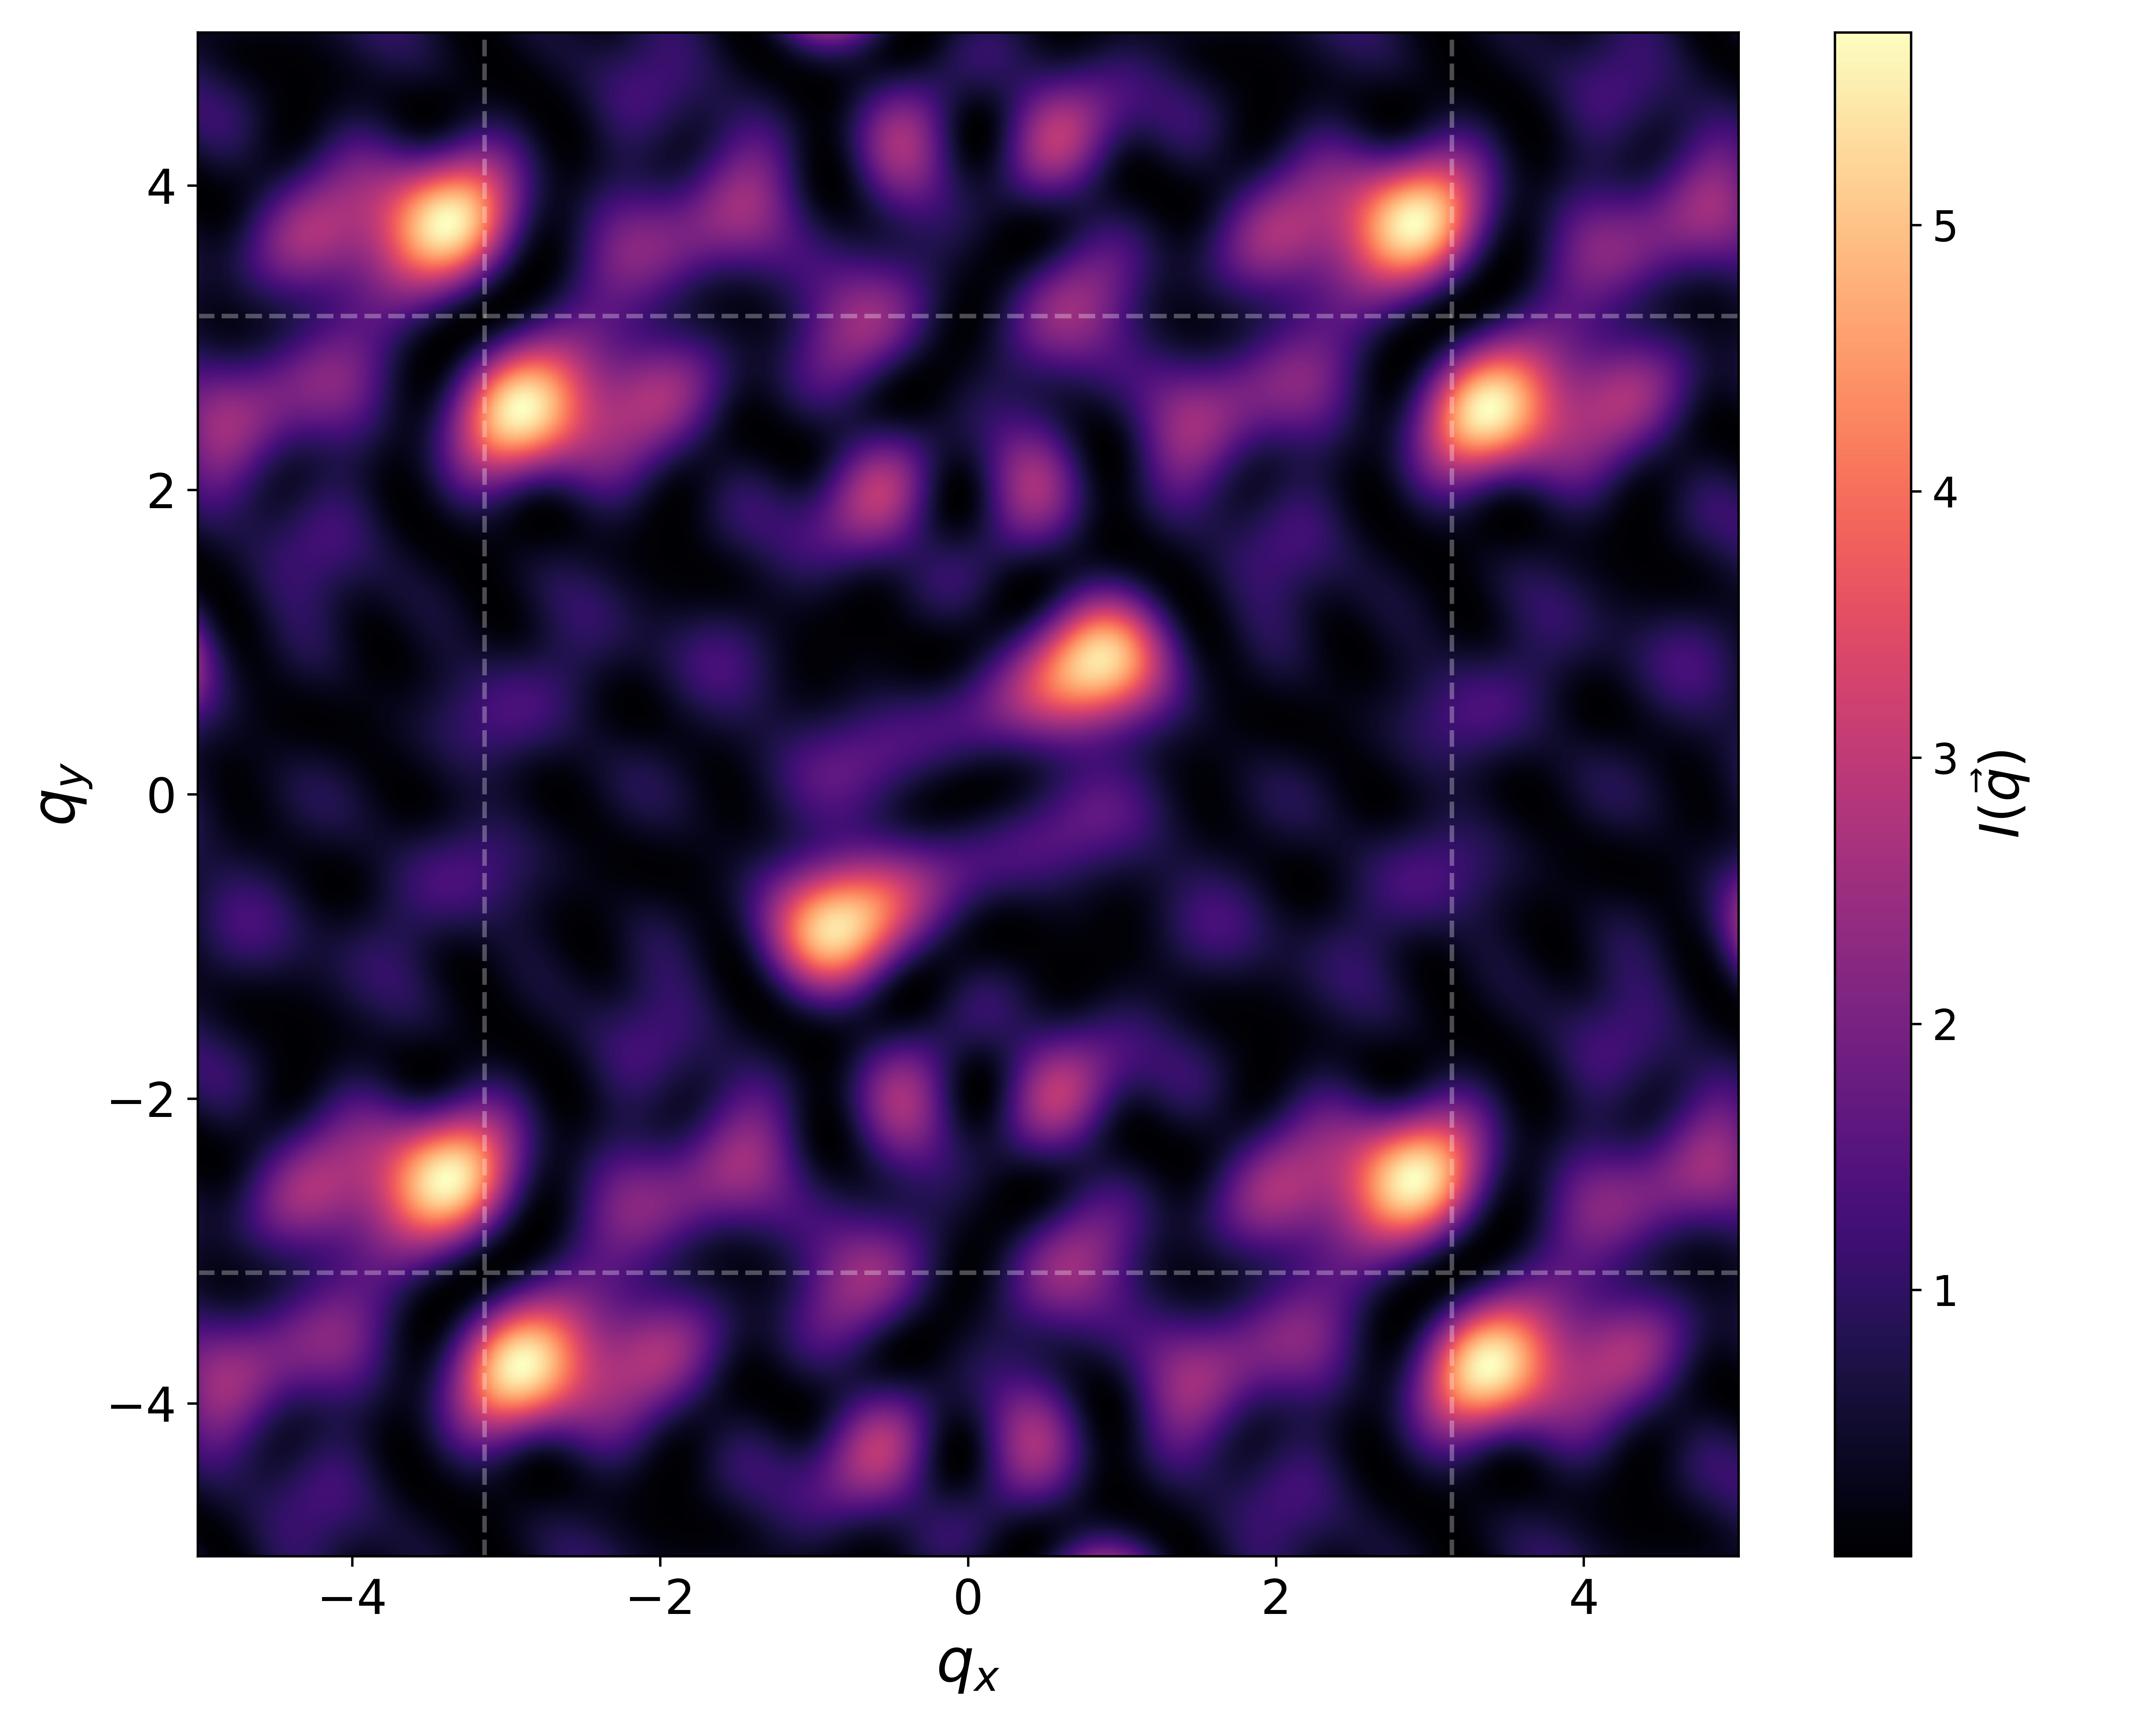
\includegraphics[width=\linewidth]{figs/cell64_J0_1_config_5_msf}
	\end{minipage}
	\hfill
	\begin{minipage}{0.5\linewidth}
		\centering
		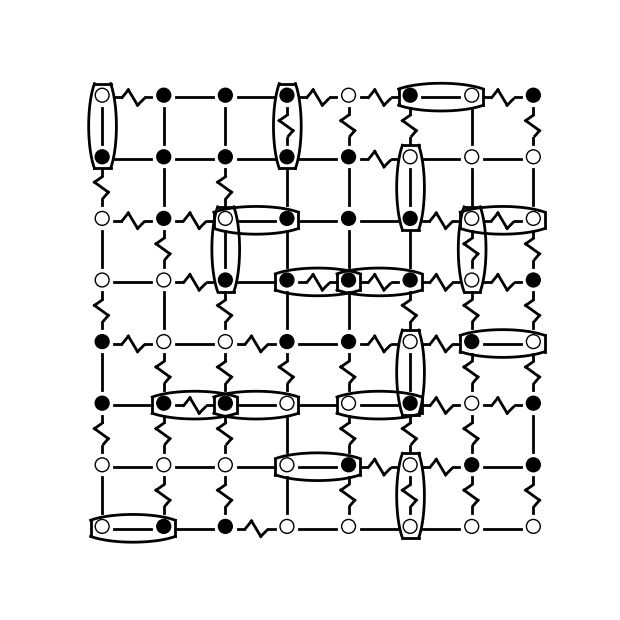
\includegraphics[width=\linewidth]{figs/cell64_J0_1_config_5}
	\end{minipage}
	\vfill
	\begin{minipage}{0.5\linewidth}
		\centering
		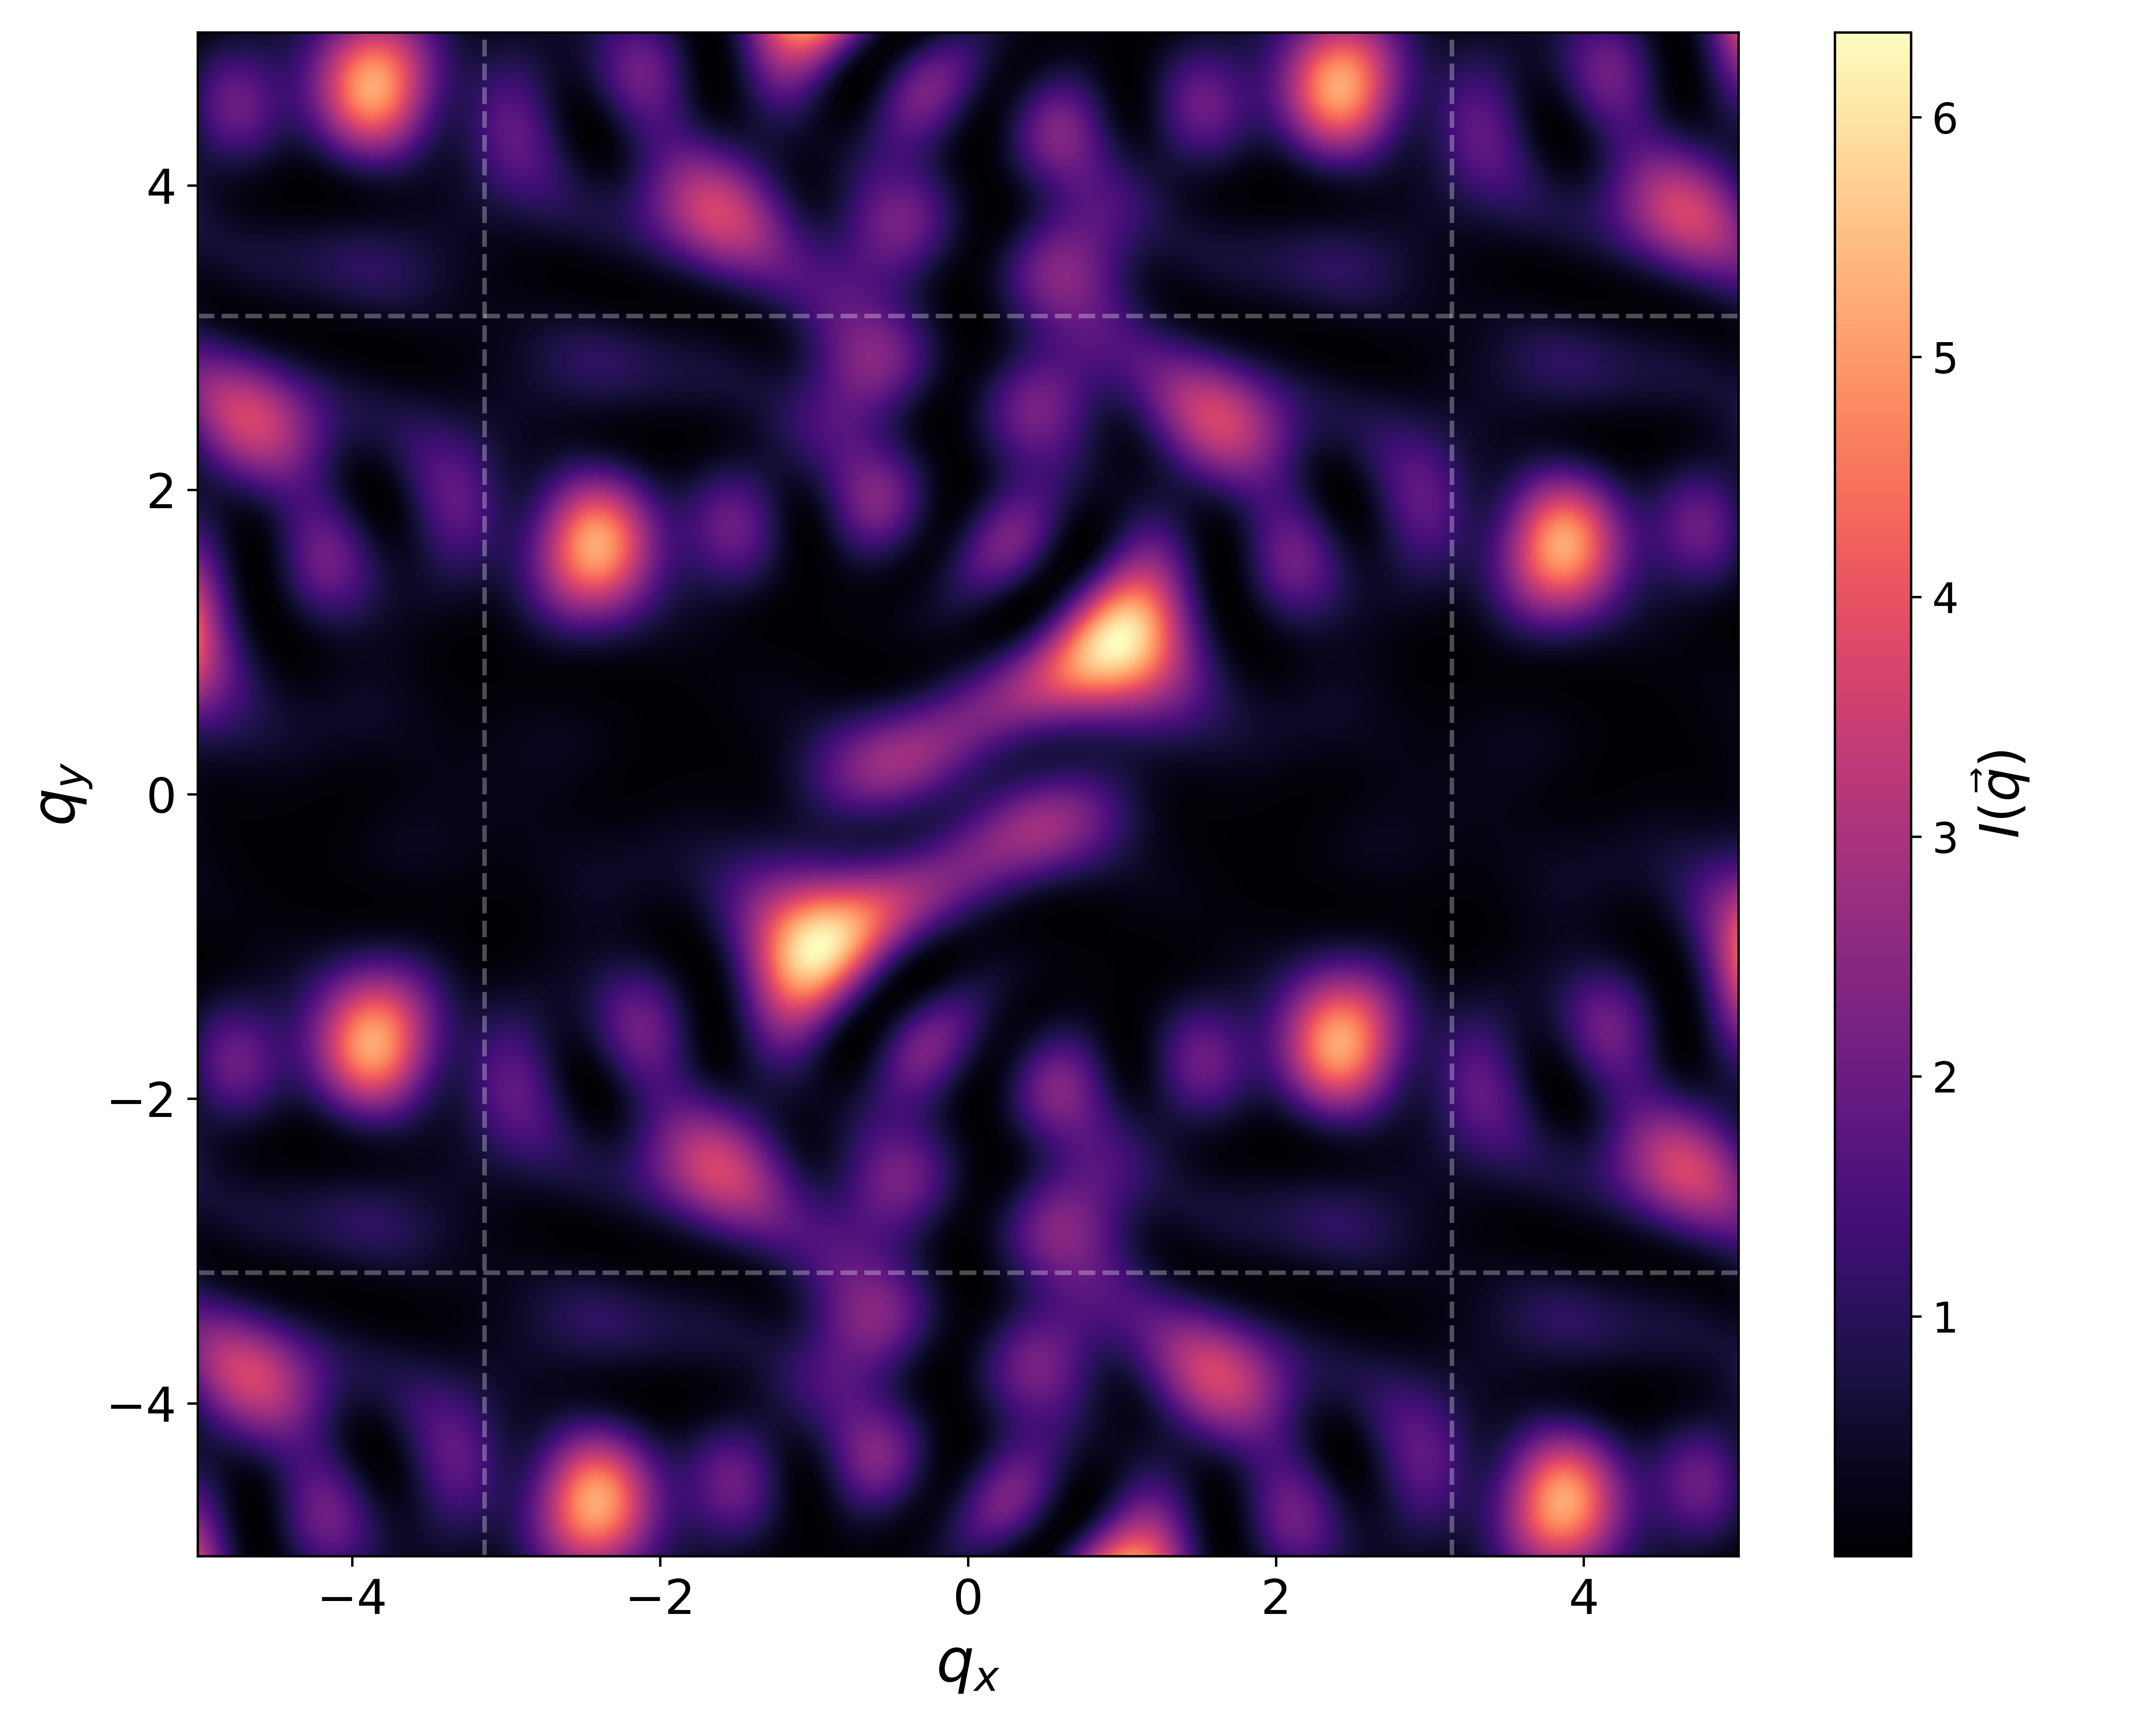
\includegraphics[width=\linewidth]{figs/cell64_J0_1_config_4_msf}
	\end{minipage}
	\hfill
	\begin{minipage}{0.5\linewidth}
		\centering
		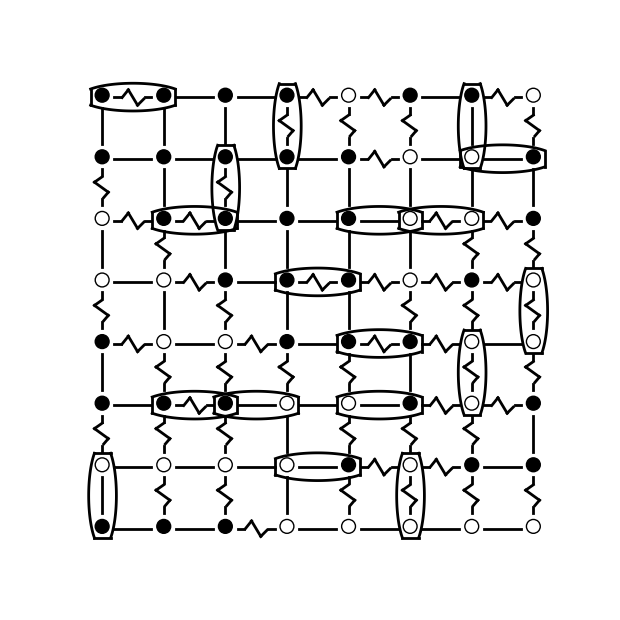
\includegraphics[width=\linewidth]{figs/cell64_J0_1_config_4}
	\end{minipage}
	\vfill
	\begin{minipage}{0.5\linewidth}
		\centering
		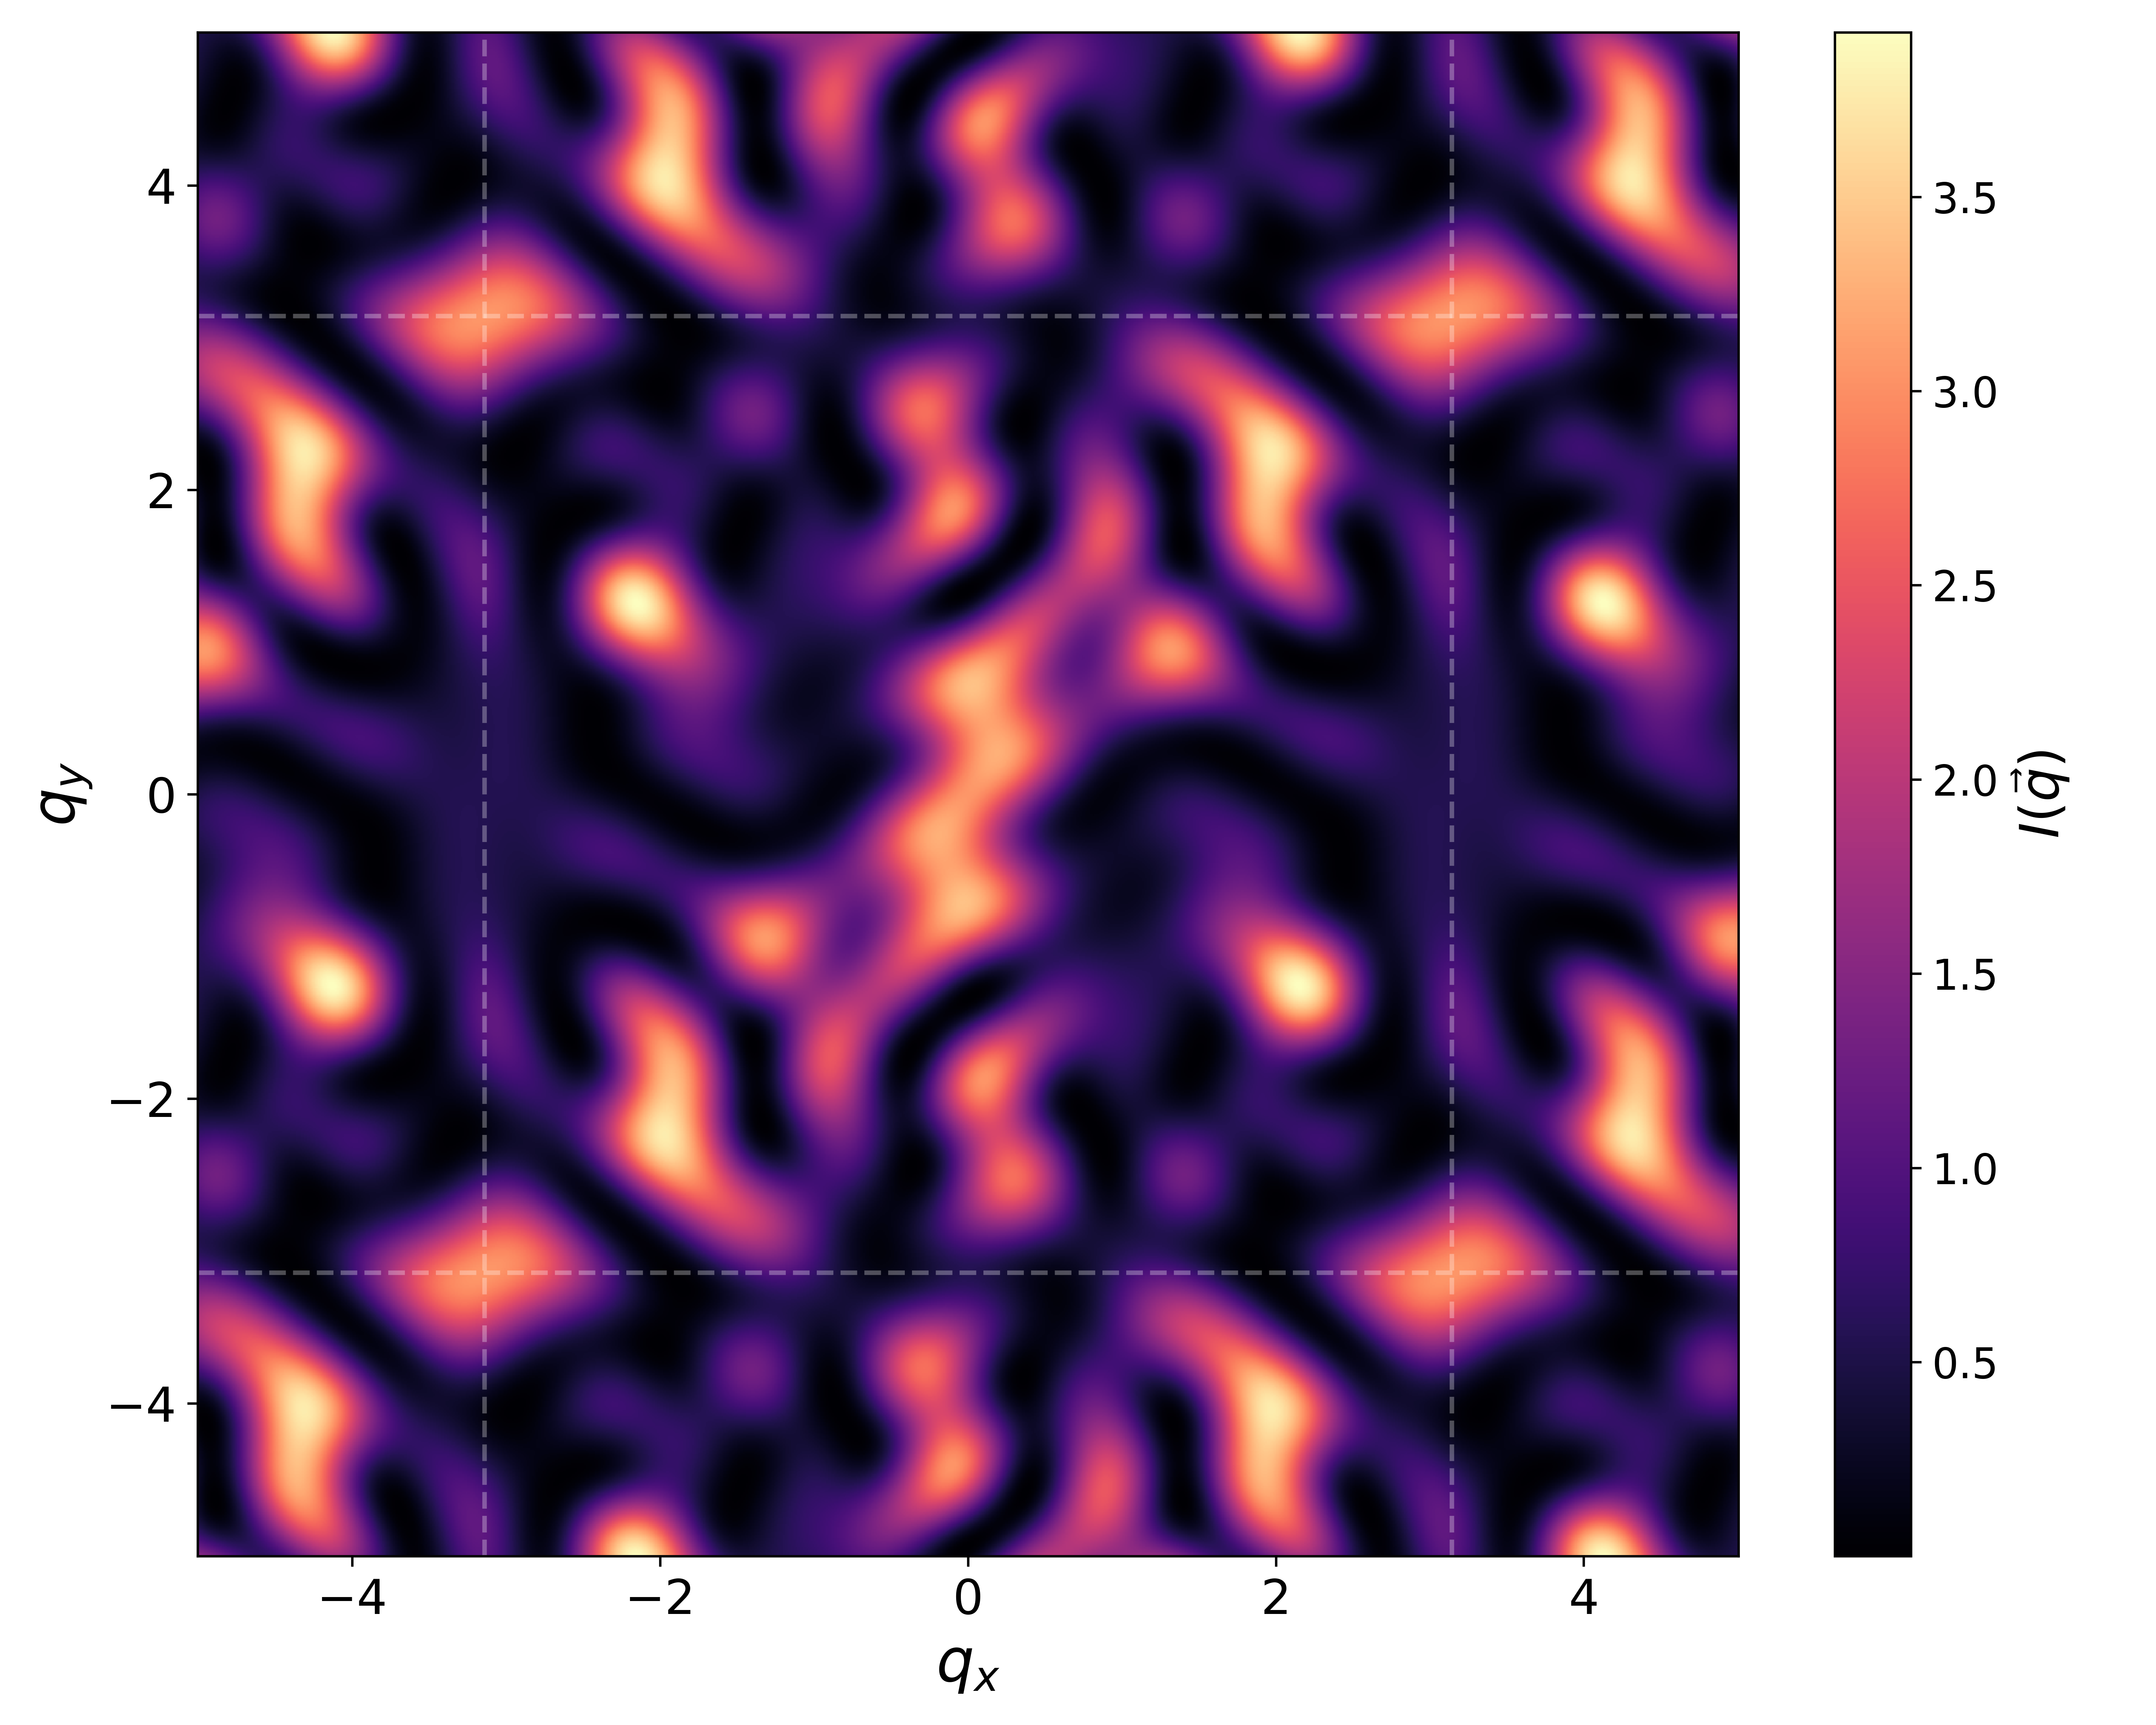
\includegraphics[width=\linewidth]{figs/cell64_J0_1_config_3_msf}
	\end{minipage}
	\hfill
	\begin{minipage}{0.5\linewidth}
		\centering
		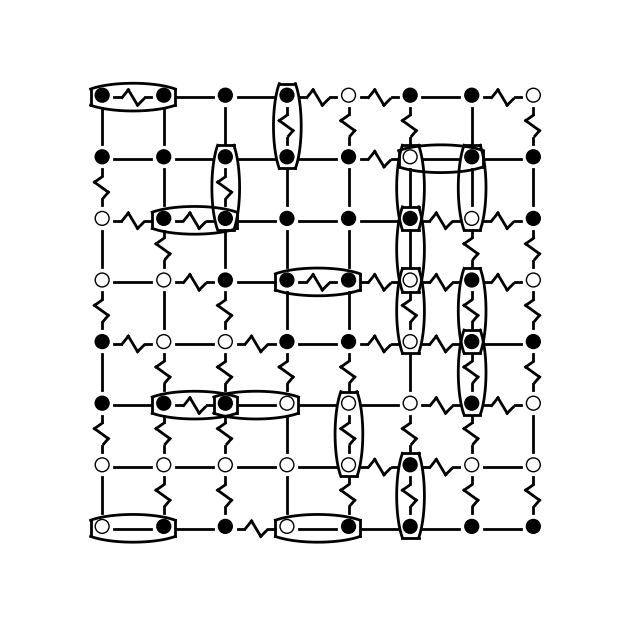
\includegraphics[width=\linewidth]{figs/cell64_J0_1_config_3}
	\end{minipage}
	\caption{Магнитный структурный фактор $I(\vec{q})$ для конфигураций вырожденного основного состояния спинового стекла Эдвардса-Андерсона ($P_+=0.5$) при разном спиновом избытке ($M_{gs}=-2,-8,-14$) слева и соответствующая конфигурация спиновых переменных справа. \textcolor{red}{cell64\_J0\_1}}
	\label{fig:msf}
\end{figure}

На рисунке \ref{fig:msf} слева изображен магнитный структурный фактор в обратном пространстве $(q_x, q_y)$ для нескольких конфигураций вырожденного основного состояния спинового стекла Эдвардса-Андерсона ($M_{gs}=-2,-8,-14$). Справа показана соответствующая $I(\vec{q})$ конфигурация спиновых переменных. Белые и черные круги - $S_i=\pm1$, прямые и зубчатые линии - ферромагнитные и антиферромагнитные связи, обведенные пары узлов - фрустрированные пары.

Так как спиновое стекло характеризуется разупорядоченным положением спинов за счет конкурирующих взаимодействий, то пики $I(\vec{q})$ в обратном пространстве размыты, расположены хаотично и отличаются для разных конфигураций спиновых переменных соответствующих одному и тому же основному состоянию. Тем не менее, на рисунке \ref{fig:msf} снизу для $I(\vec{q})$ при $|M_{gs}| = 14$ мы можем видеть, что помимо большого количества хаотично расположенных пятен, также наблюдается пятна в точках $(\pm\pi,\pm\pi)$ и продолговатая область с высоким значением $I(\vec{q})$ и центром в точке $(0,0)$. То есть в каком-то виде происходит ферро- и антиферромагнитное упорядочение одновременно. Это является следствием того, что в конфигурации основного состояния спинового стекла образуются ферромагнитные и антиферромагнитные кластеры.

\begin{figure}[H]
	\begin{minipage}{0.5\linewidth}
		\centering
		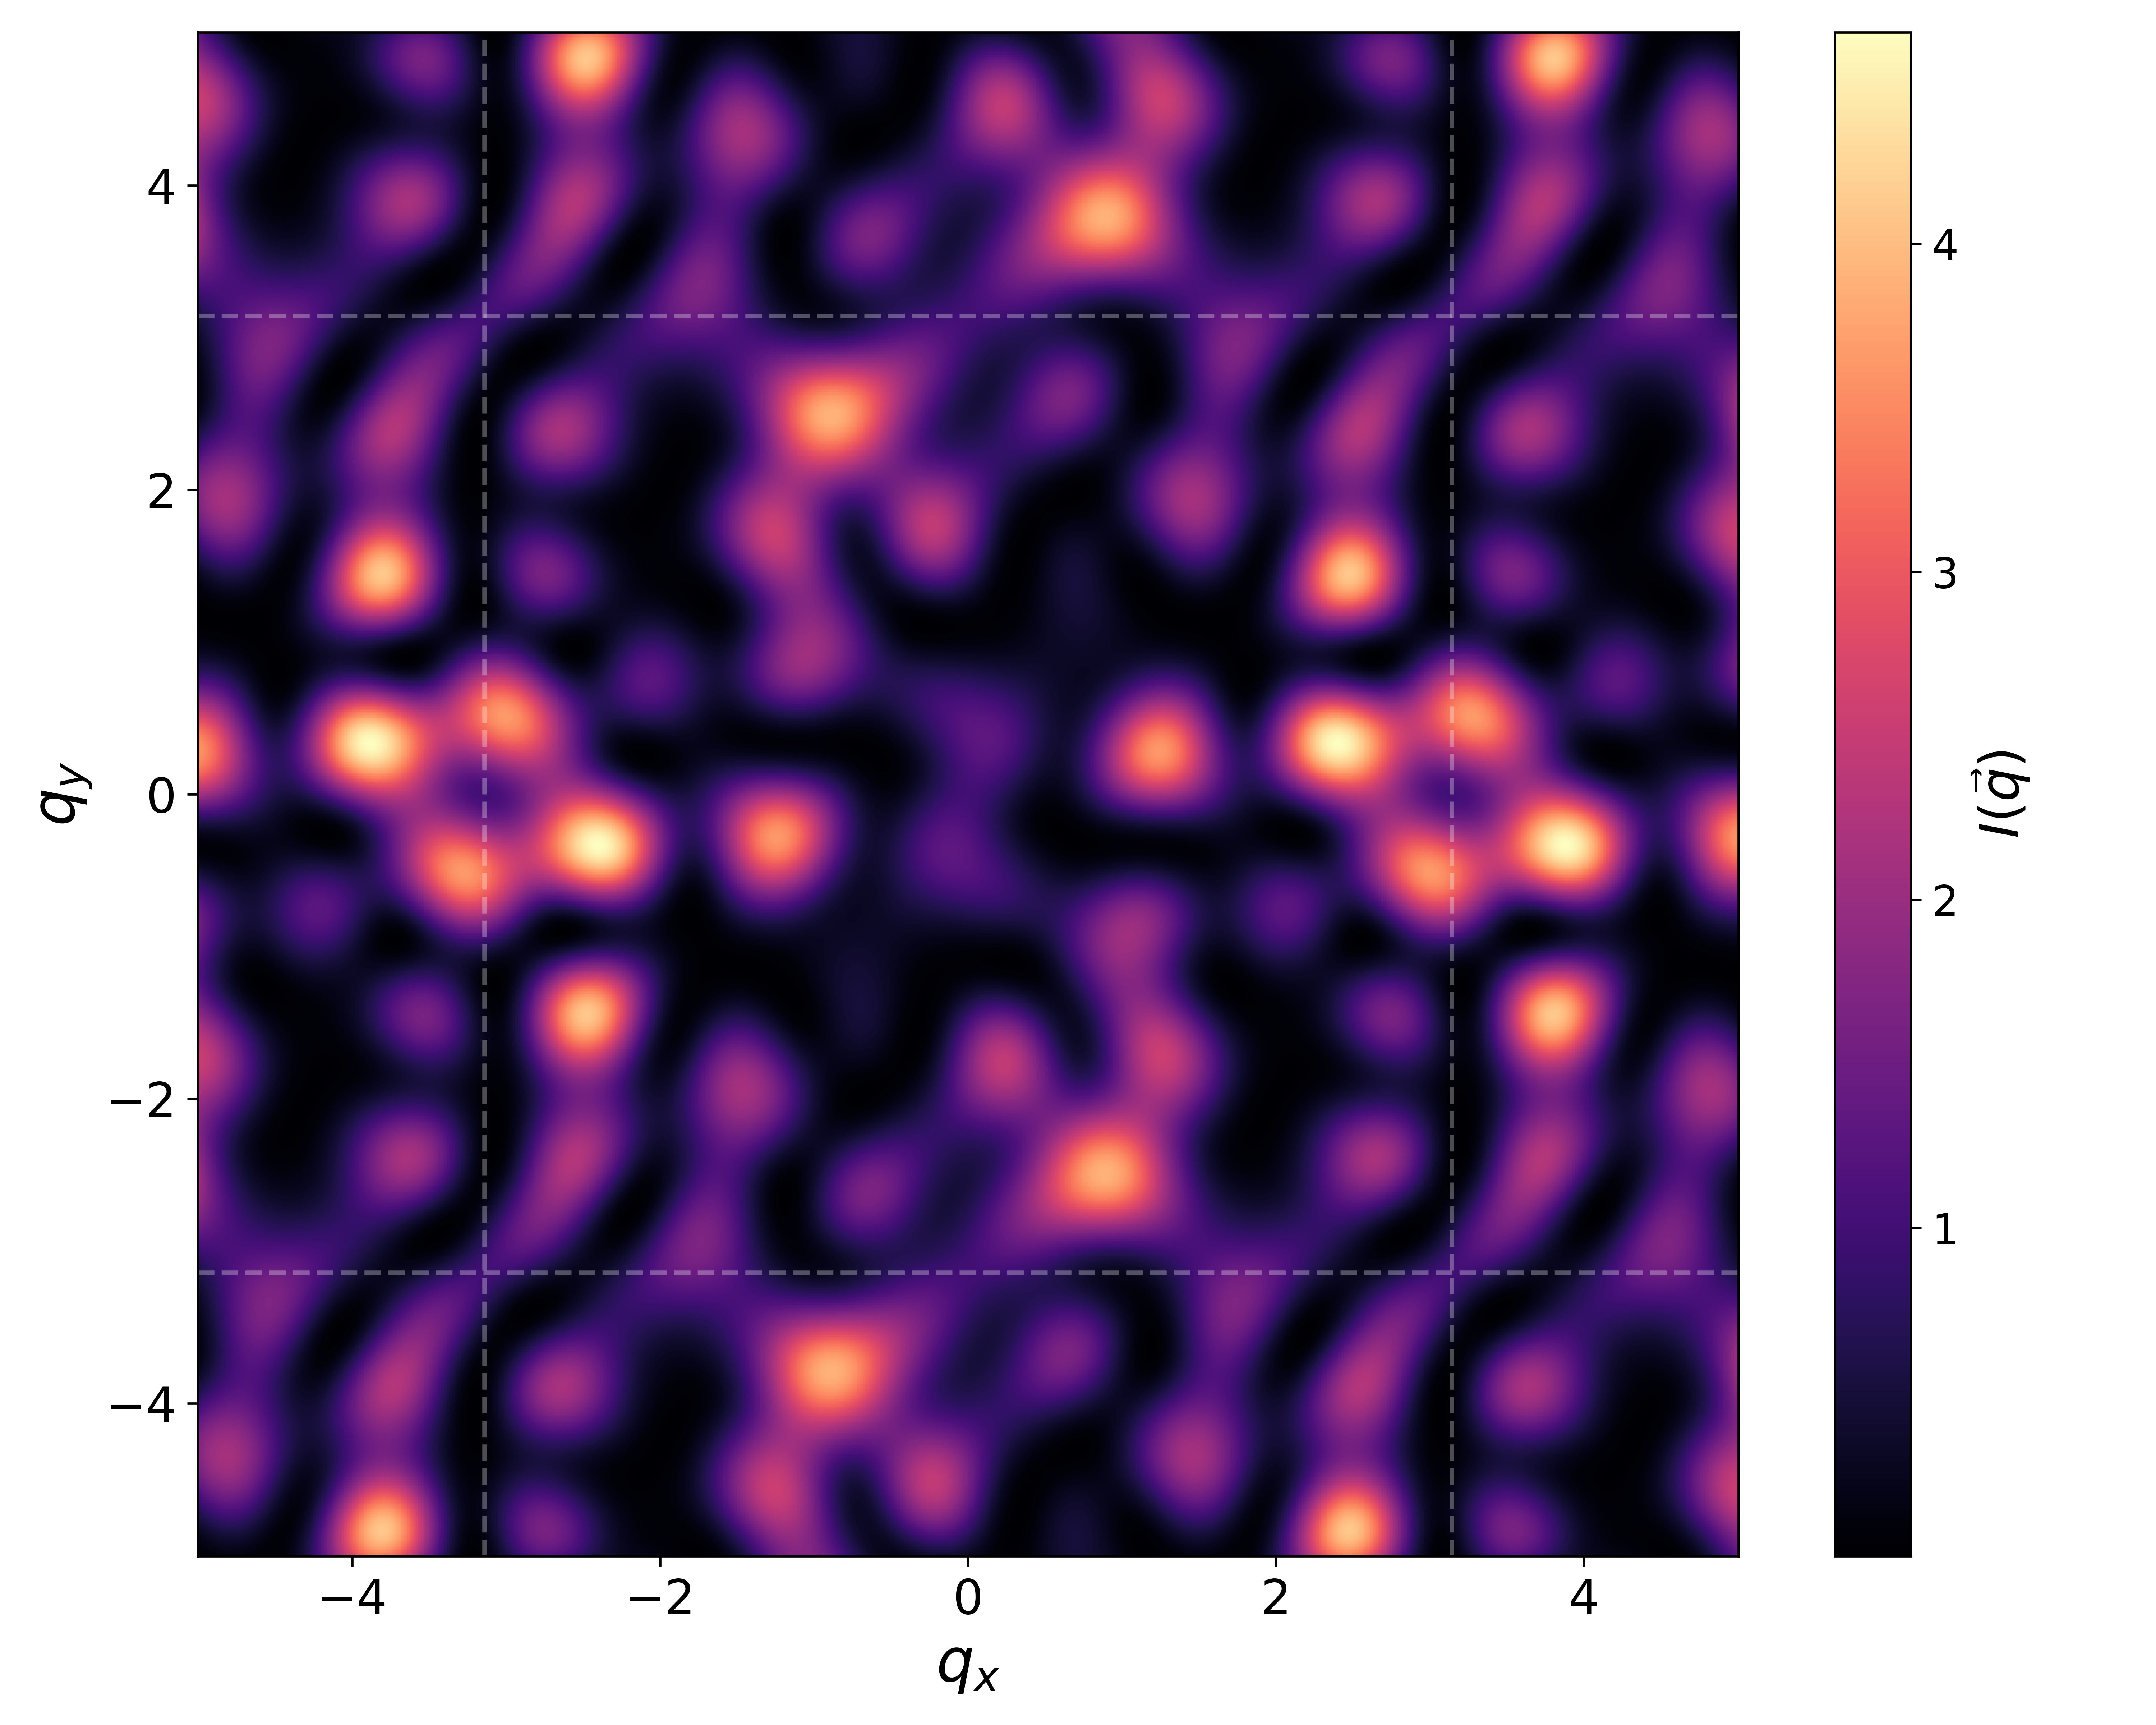
\includegraphics[width=\linewidth]{figs/cell64_J0_8_config_1_msf}
	\end{minipage}
	\hfill
	\begin{minipage}{0.5\linewidth}
		\centering
		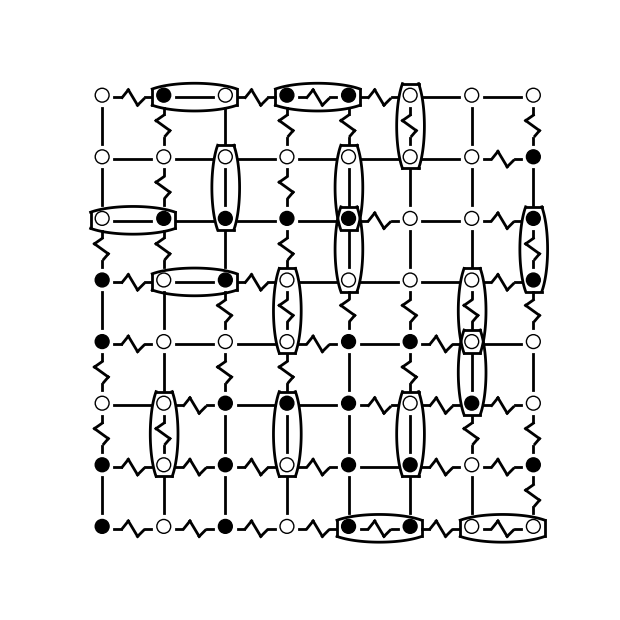
\includegraphics[width=\linewidth]{figs/cell64_J0_8_config_1}
	\end{minipage}
	\vfill
	\begin{minipage}{0.5\linewidth}
		\centering
		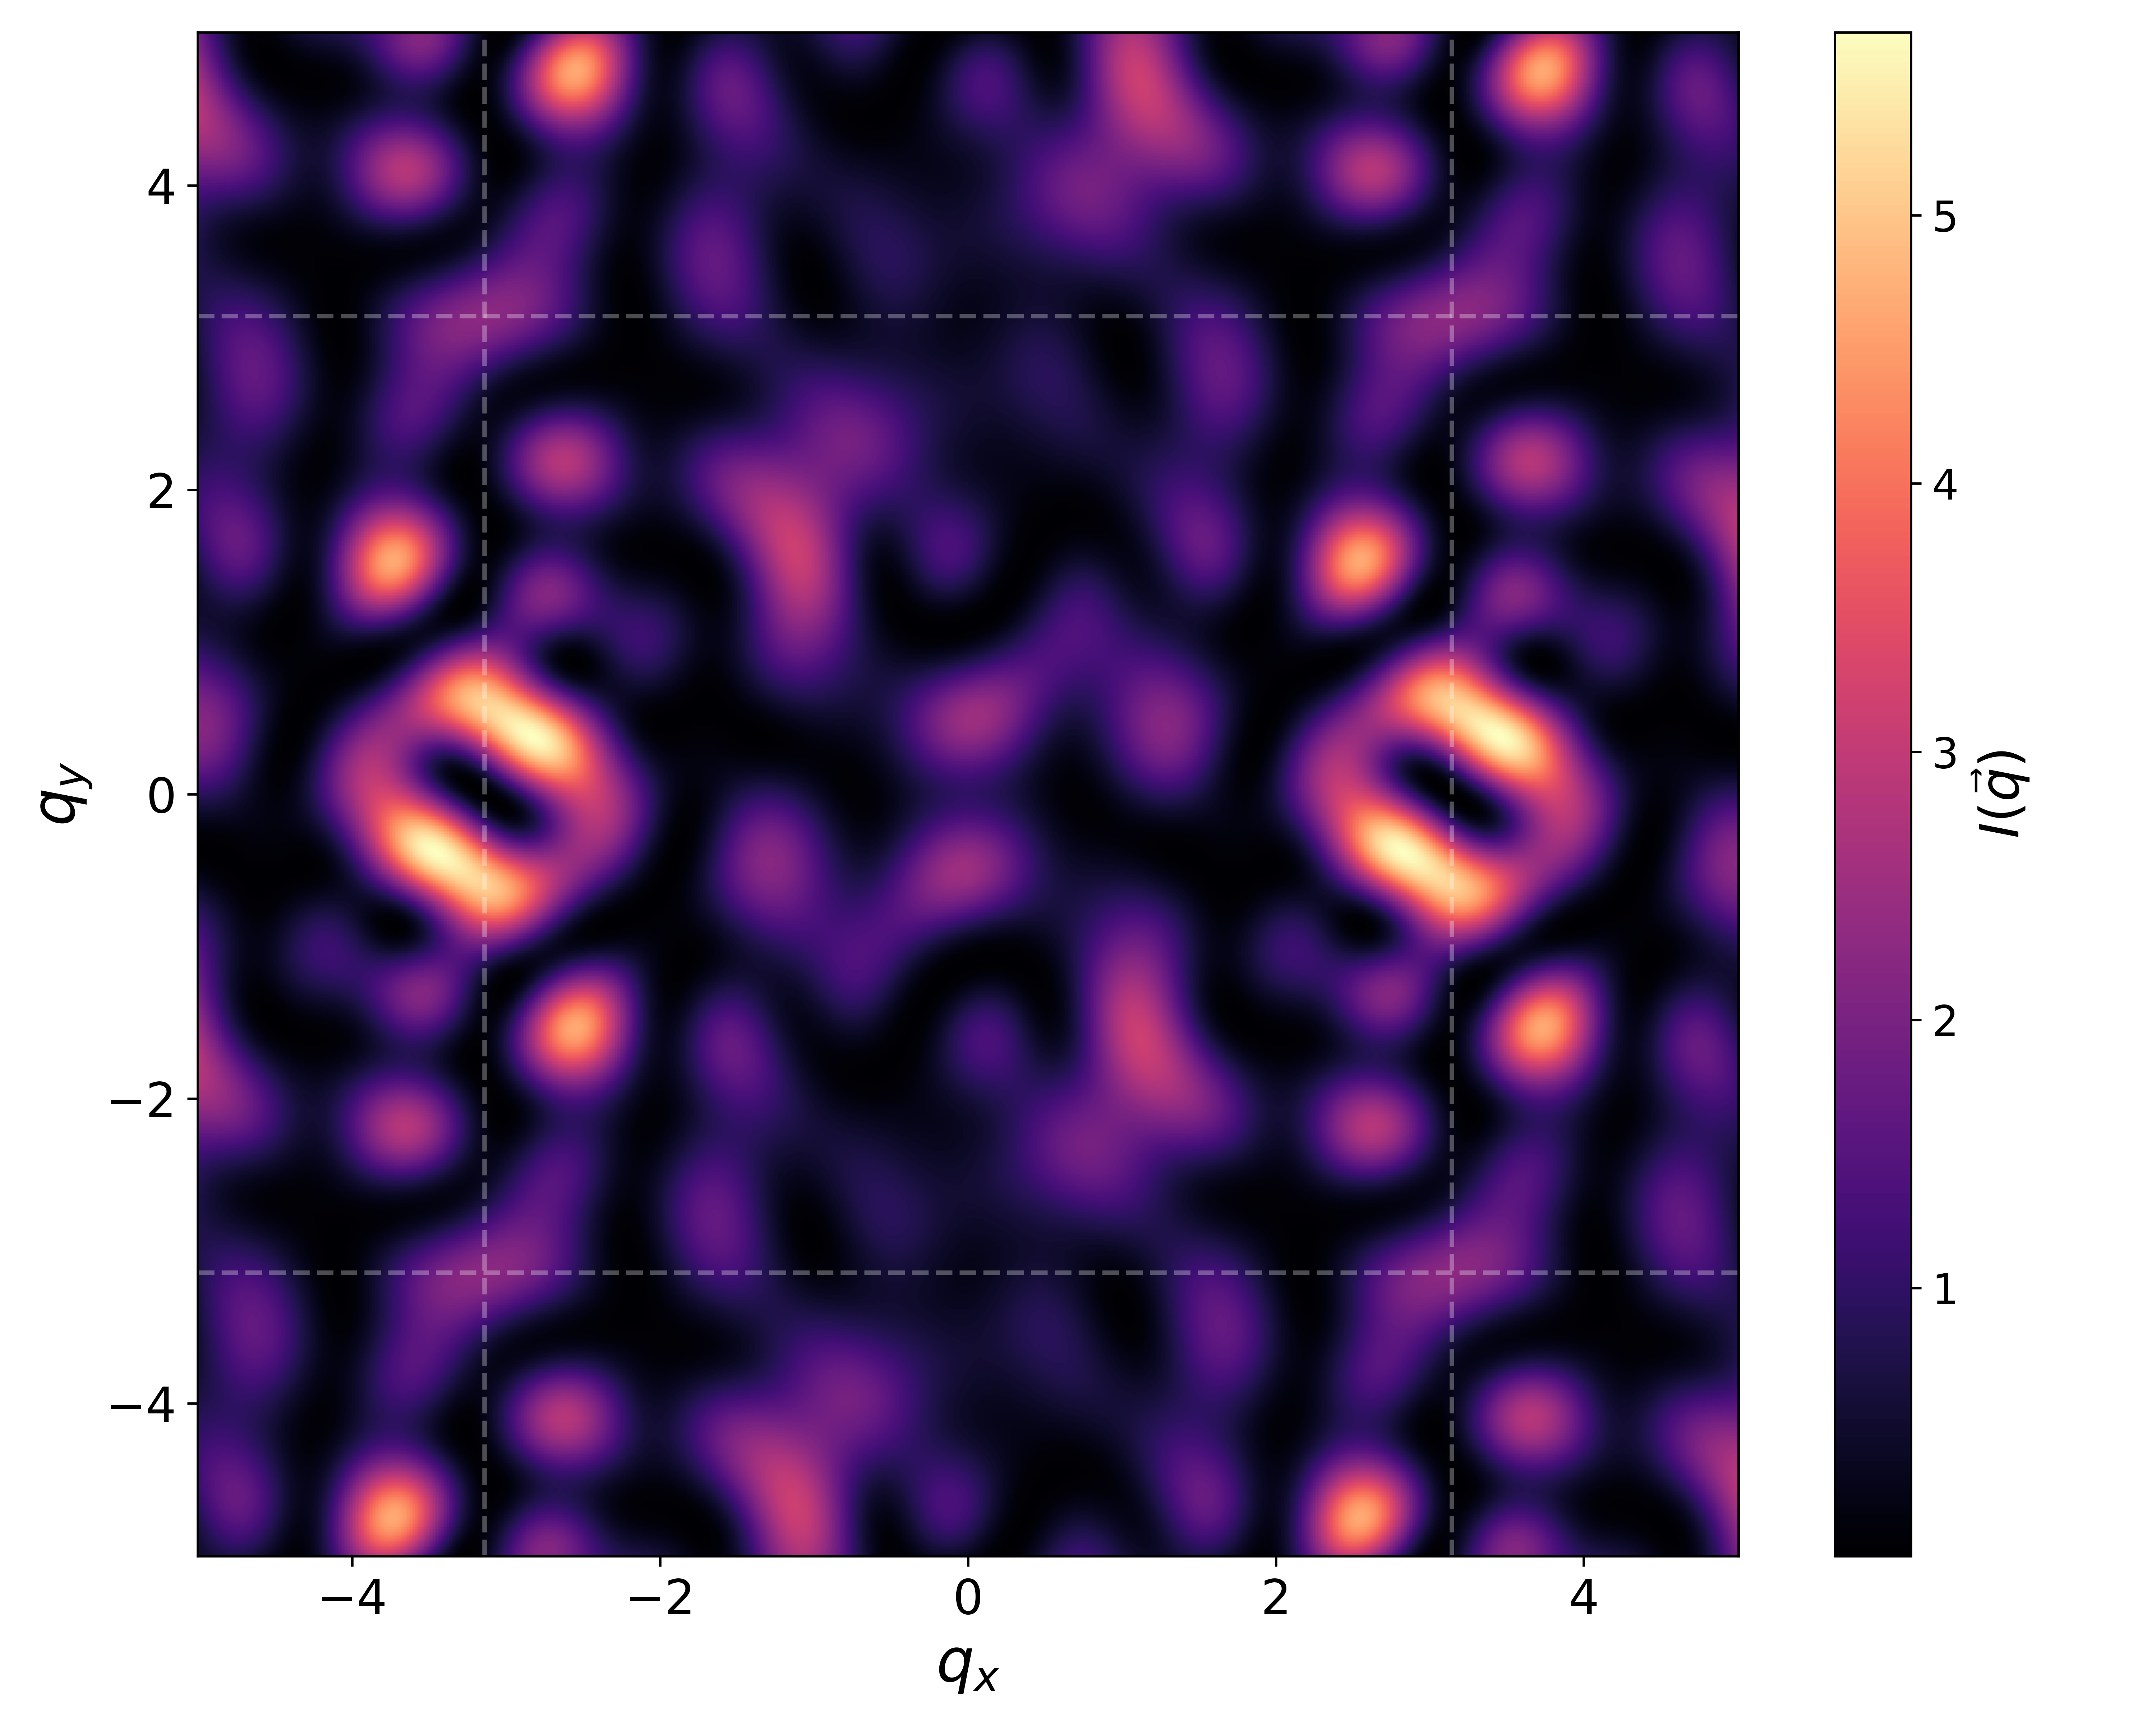
\includegraphics[width=\linewidth]{figs/cell64_J0_8_config_2_msf}
	\end{minipage}
	\hfill
	\begin{minipage}{0.5\linewidth}
		\centering
		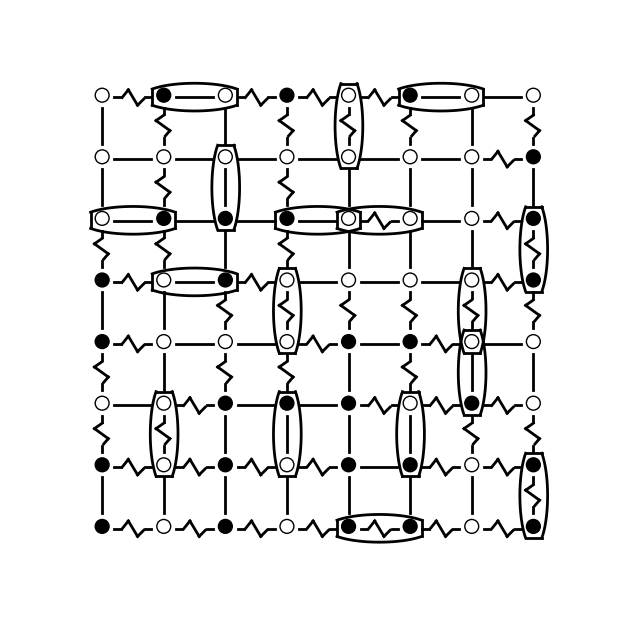
\includegraphics[width=\linewidth]{figs/cell64_J0_8_config_2}
	\end{minipage}
	\vfill
	\begin{minipage}{0.5\linewidth}
		\centering
		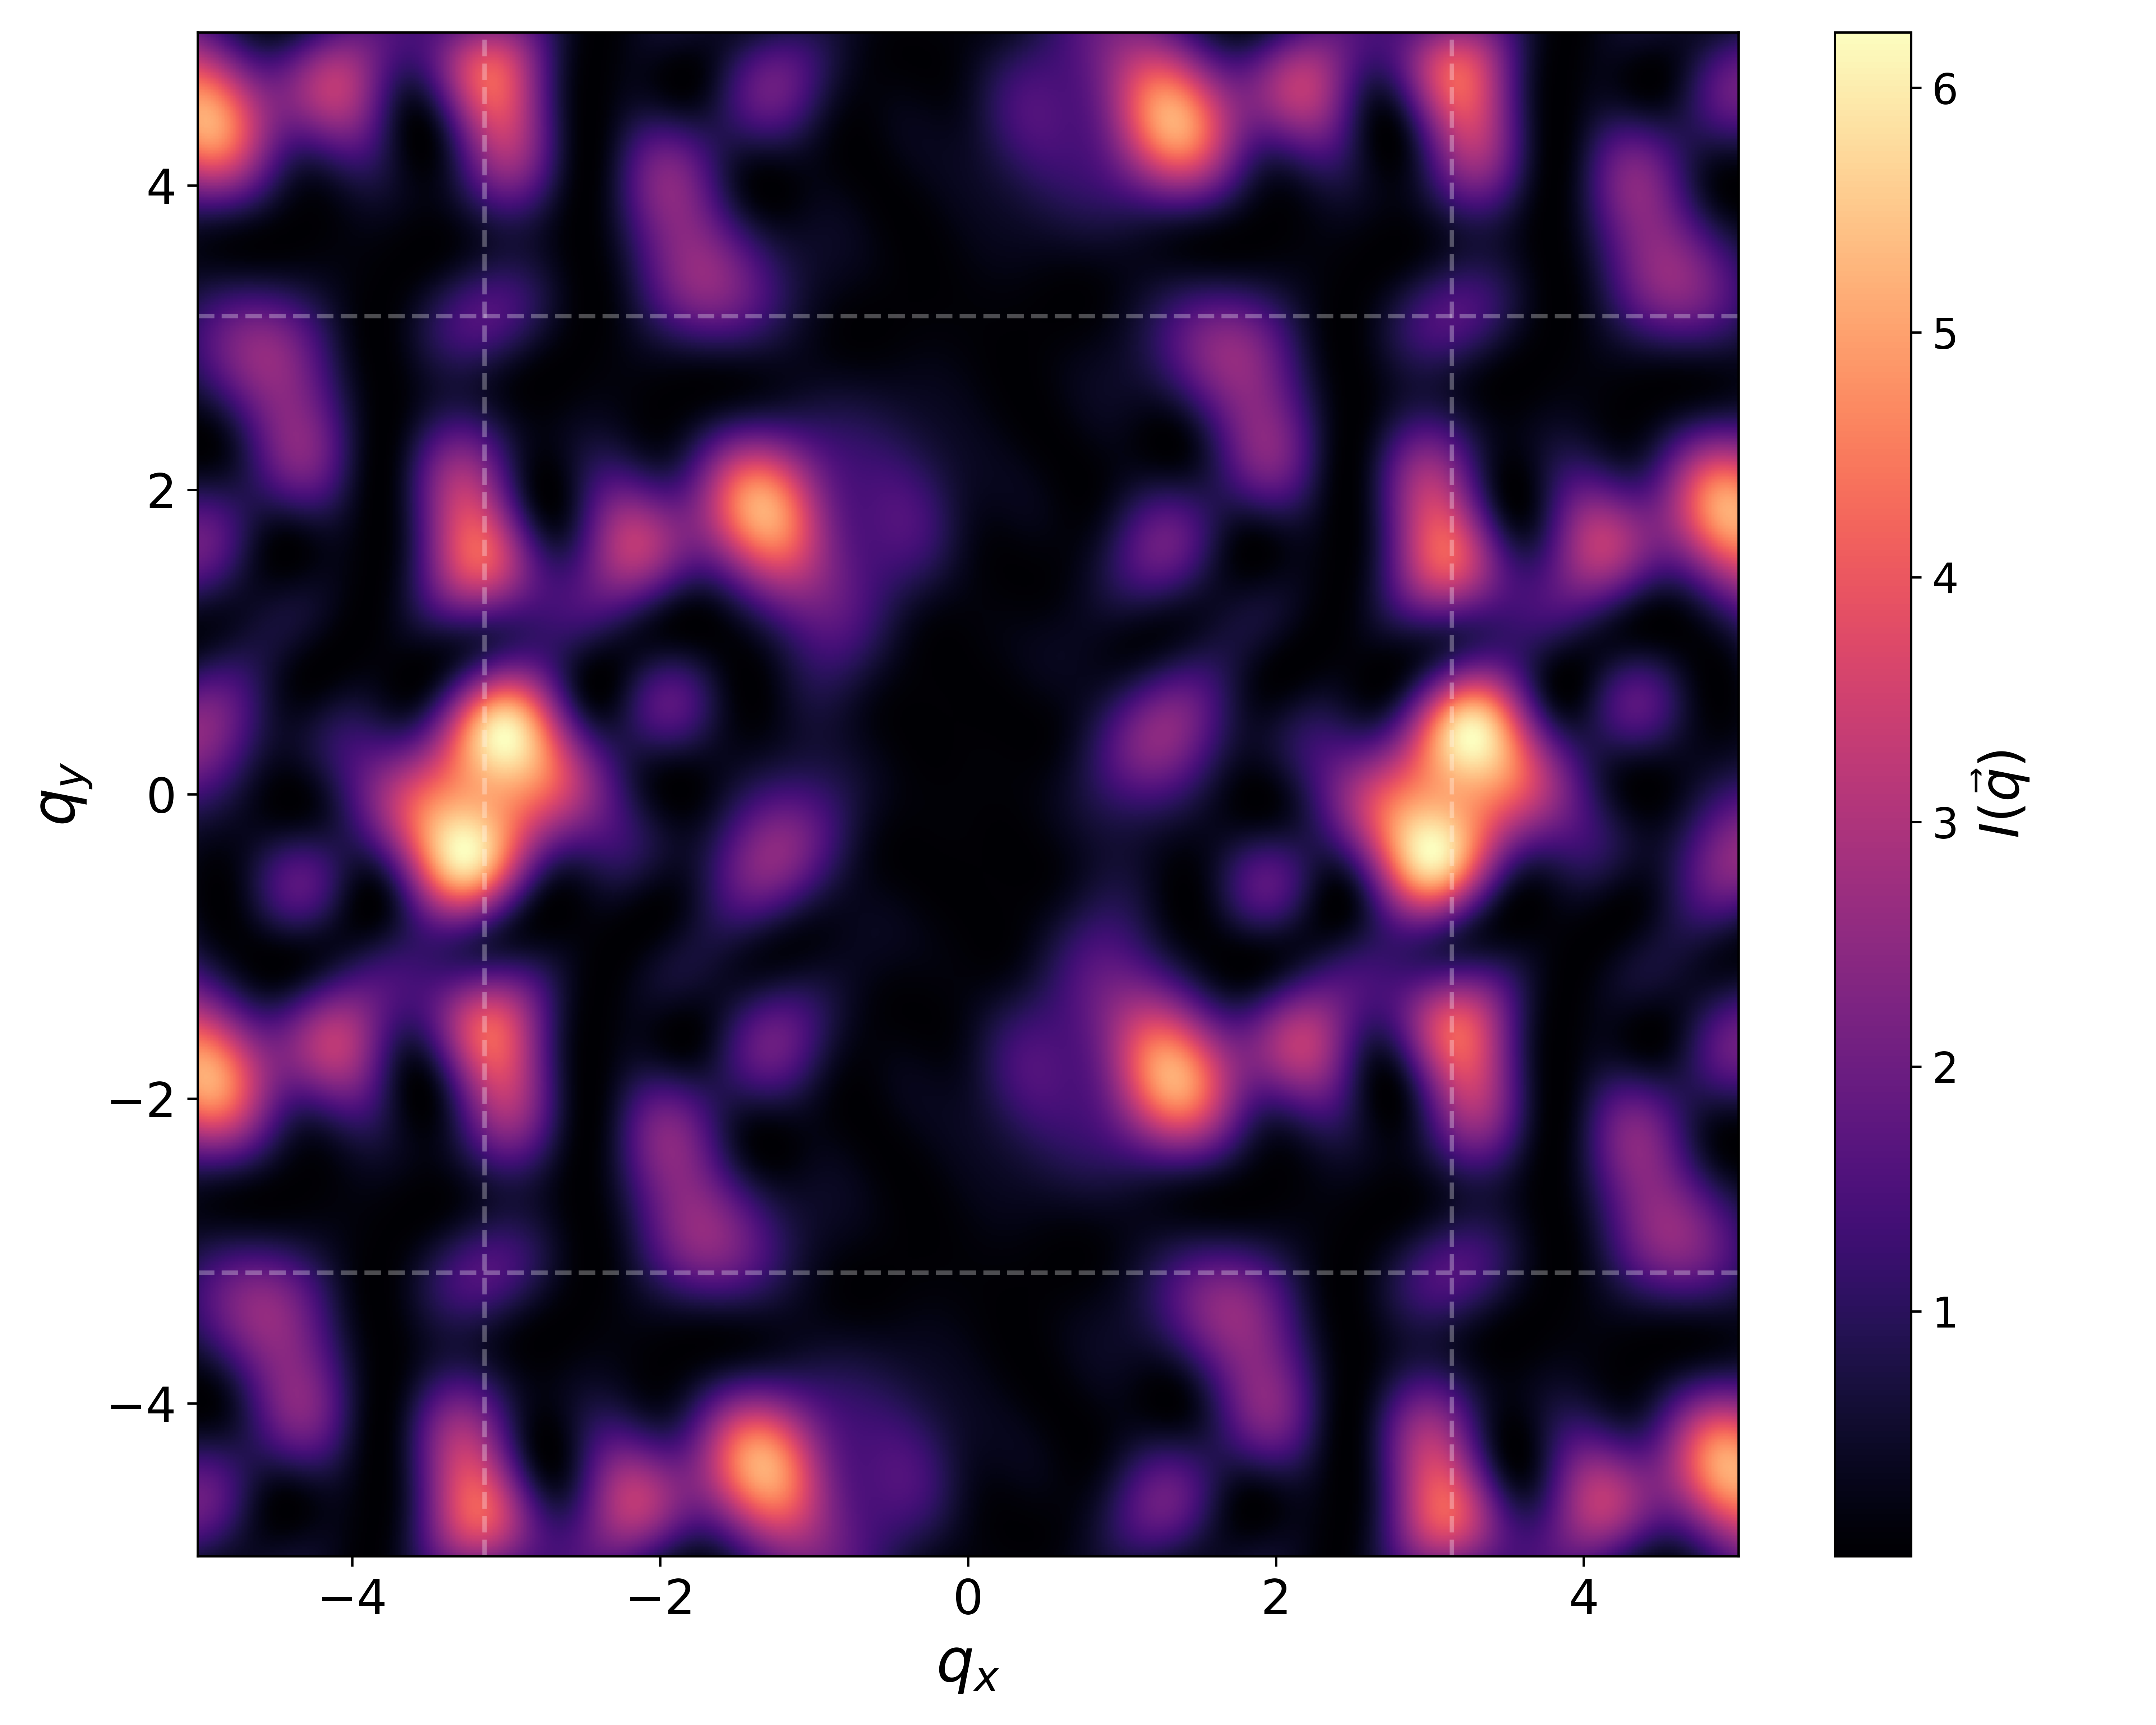
\includegraphics[width=\linewidth]{figs/cell64_J0_8_config_5_msf}
	\end{minipage}
	\hfill
	\begin{minipage}{0.5\linewidth}
		\centering
		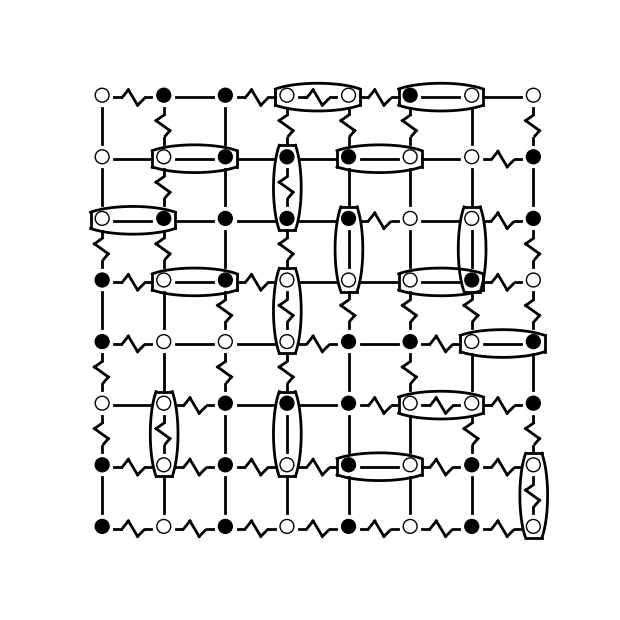
\includegraphics[width=\linewidth]{figs/cell64_J0_8_config_5}
	\end{minipage}
	\caption{\textcolor{red}{cell64\_J0\_8 $M_{gs} = 8, 8, 2$}}
	\label{fig:ms2}
\end{figure}


\section{Заключение}


Текст заключения.


\section{Благодарности}

Исследование выполнено за счет гранта Российского научного фонда № 24-71-10069, https://rscf.ru/project/24-71-10069/.

The research was supported by the Russian Science Foundation grant No. 24-71-10069, https://rscf.ru/en/project/24-71-10069/.

\bibliography{mybibfile.bib}


\end{document}